% DO NOT COMPILE THIS FILE DIRECTLY!
% This is included by the other .tex files.

\begin{frame}[t,plain]
\titlepage
\end{frame}

\begin{frame}
    \frametitle{\texttt{\$ whoarewe}}
    \begin{center}
        
\includegraphics[width=0.25\linewidth]{pictures/whoarewe-andras.png}
        \qquad
        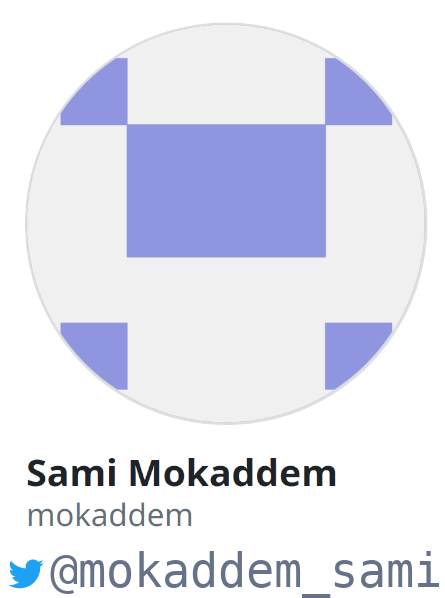
\includegraphics[width=0.25\linewidth]{pictures/whoarewe-sami.png}
    \end{center}
    \vspace{0.5em}
    \begin{center}
        \frame{
\includegraphics[width=0.45\linewidth]{pictures/something-stupid.jpeg}}
    \end{center}
\end{frame}

\begin{frame}
    \frametitle{Agenda}
    \vspace{-3em}
    \begin{center}
        
\includegraphics[width=0.65\linewidth]{pictures/fun-begin.jpeg}
    \end{center}
    \begin{itemize}
        \item Why MISP 3?
        \item The plan
        \item Considerations
    \end{itemize}
\end{frame}

\section{Why MISP 3?}
\begin{frame}
    \frametitle{> An outdated version of the framework}
    \begin{center}
        
\includegraphics[width=0.3\linewidth]{pictures/cakephp.png}
    \end{center}
    \begin{itemize}
        \item MISP is based on CakePHP 2.x
        \begin{itemize}
            \item End of Security Support in {\bf June 2021}
            \item Maintained fork github.com:MISP/cakephp.git
        \end{itemize}
        \item CakePHP supports PHP version {\bf <=7.4}
        \begin{itemize}
            \item End of Security Support in {\bf November 2022}
        \end{itemize}
    \end{itemize}
    % \begin{center}
    %     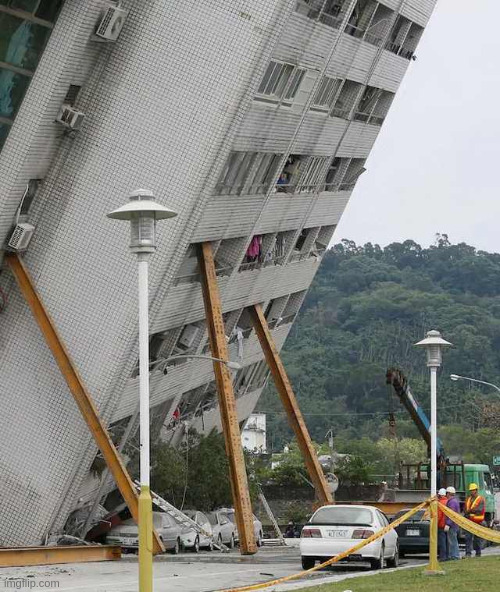
\includegraphics[width=0.2\linewidth]{pictures/building-collapse.jpeg}
    % \end{center}
    \begin{center}
        
\includegraphics[width=0.5\linewidth]{pictures/this-is-fine.jpg}
    \end{center}
\end{frame}

\begin{frame}[fragile]
    \frametitle{> Tacked on mechanics}
    \vspace{1em}
    \begin{minipage}{0.7\textwidth}
        \begin{itemize}
            \item MISP supports a wide range of use cases...
            \item ... meaning loads of feature-clutter the interface
            \item All options visible regardless of the user profile
            \item Lack of coherent page navigation
        \end{itemize}
    \end{minipage}%
    \begin{minipage}{0.3\textwidth}
        \begin{center}
            \;\;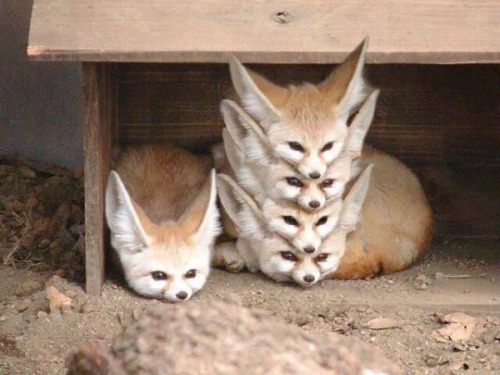
\includegraphics[width=0.8\linewidth]{pictures/fennec-stack.png}
        \end{center}
    \end{minipage}
    \begin{center}
        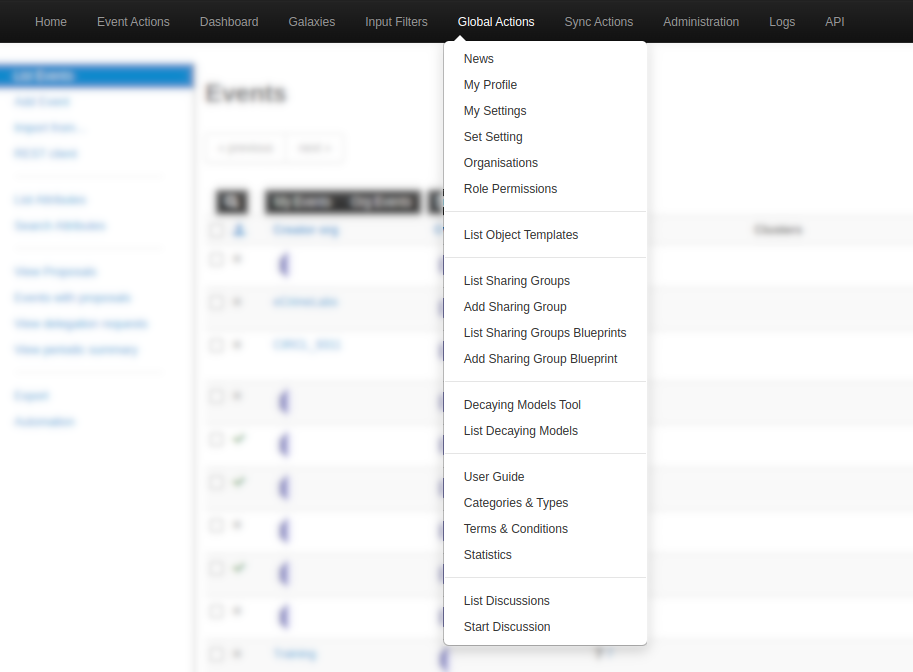
\includegraphics[width=0.55\linewidth]{pictures/confusing-navigation.png}
    \end{center}
\end{frame}

\begin{frame}
    \frametitle{> Shortcomings due to initial design choices}
    To list a few..
    \begin{itemize}
        \item Sub-optimal database structure
        \item Start with something small, build it out has its disadvantages
        \begin{itemize}
            \item Attribute \texttt{type}, \texttt{value} not a first-class citizen
            \item Logs all in one place
            \item Indexing rework (performance and moving validation to the DB)
        \end{itemize}
        \item Confusing mess of multiple graphing interfaces
        \item Files - Especially tricky with dockerised and load balanced setups
        \item Tagging
    \end{itemize}
    \begin{center}
        
\includegraphics[width=0.5\linewidth]{pictures/where-tags-objects.jpeg}
    \end{center}
\end{frame}

\begin{frame}
    \frametitle{> The \underline{ongoing} plan forward}
    \begin{itemize}
        \item Port of the codebase to a new stack
        \begin{itemize}
            \item CakePHP 2.x $\rightarrow$ CakePHP 5
        \end{itemize}
        \item Rework of old baggage
        \begin{itemize}
            \item Database updates
            \item Front-end libraries (Bootstrap, Graphing, ...)
            \item Background jobs \& Scheduled tasks
            \item Purging old libraries
        \end{itemize}
    \end{itemize}
\end{frame}

\begin{frame}
    \frametitle{> Pruning unused / dead end functionalities}
    \begin{minipage}{0.7\textwidth}
        \begin{itemize}
            \item Populate using the templating system
            \item Deprecated export functionalities
            \item Discussion / Posts
            \item $\cdots$
        \end{itemize}
    \end{minipage}%
    \begin{minipage}{0.3\textwidth}
        \begin{center}
            \;\;
\includegraphics[width=1\linewidth]{pictures/we-want-you.jpeg}
        \end{center}
    \end{minipage}
    
\end{frame}

\section{Step I - Preparing the grounds}
\begin{frame}
    \frametitle{Step I - Preparing the grounds}
    Refactoring the codebase for improved portability using factories
    \begin{itemize}
        \item Framework-agnostic
        \item Reusable code for front and back-end
        \item Extracting and encapsulating specialised functionalities into libraries
    \end{itemize}
\end{frame}


\begin{frame}
    \frametitle{Step I - Preparing the grounds}
    \vspace{-2em}
    \begin{center}
        
\includegraphics[width=0.2\linewidth]{pictures/cerebrate.png}
    \end{center}
    Setting the stage with Cerebrate
    \begin{itemize}
        \item Dev started in May 2020, built on MISP3's stack
        \item Application built on top of ported MISP libraries
        \item New UI laying the foundation for MISP 3
        \item Streamlined integration of new features into MISP3
        \vspace{-0.5em}
        \begin{itemize}
            \item Tagging, Inbox system, Settings, $\cdots$
        \end{itemize}
    \end{itemize}
\end{frame}

\begin{frame}
    \frametitle{Step I - Identifying inter-dependencies}
    Migrate least connected part first
    \begin{center}
        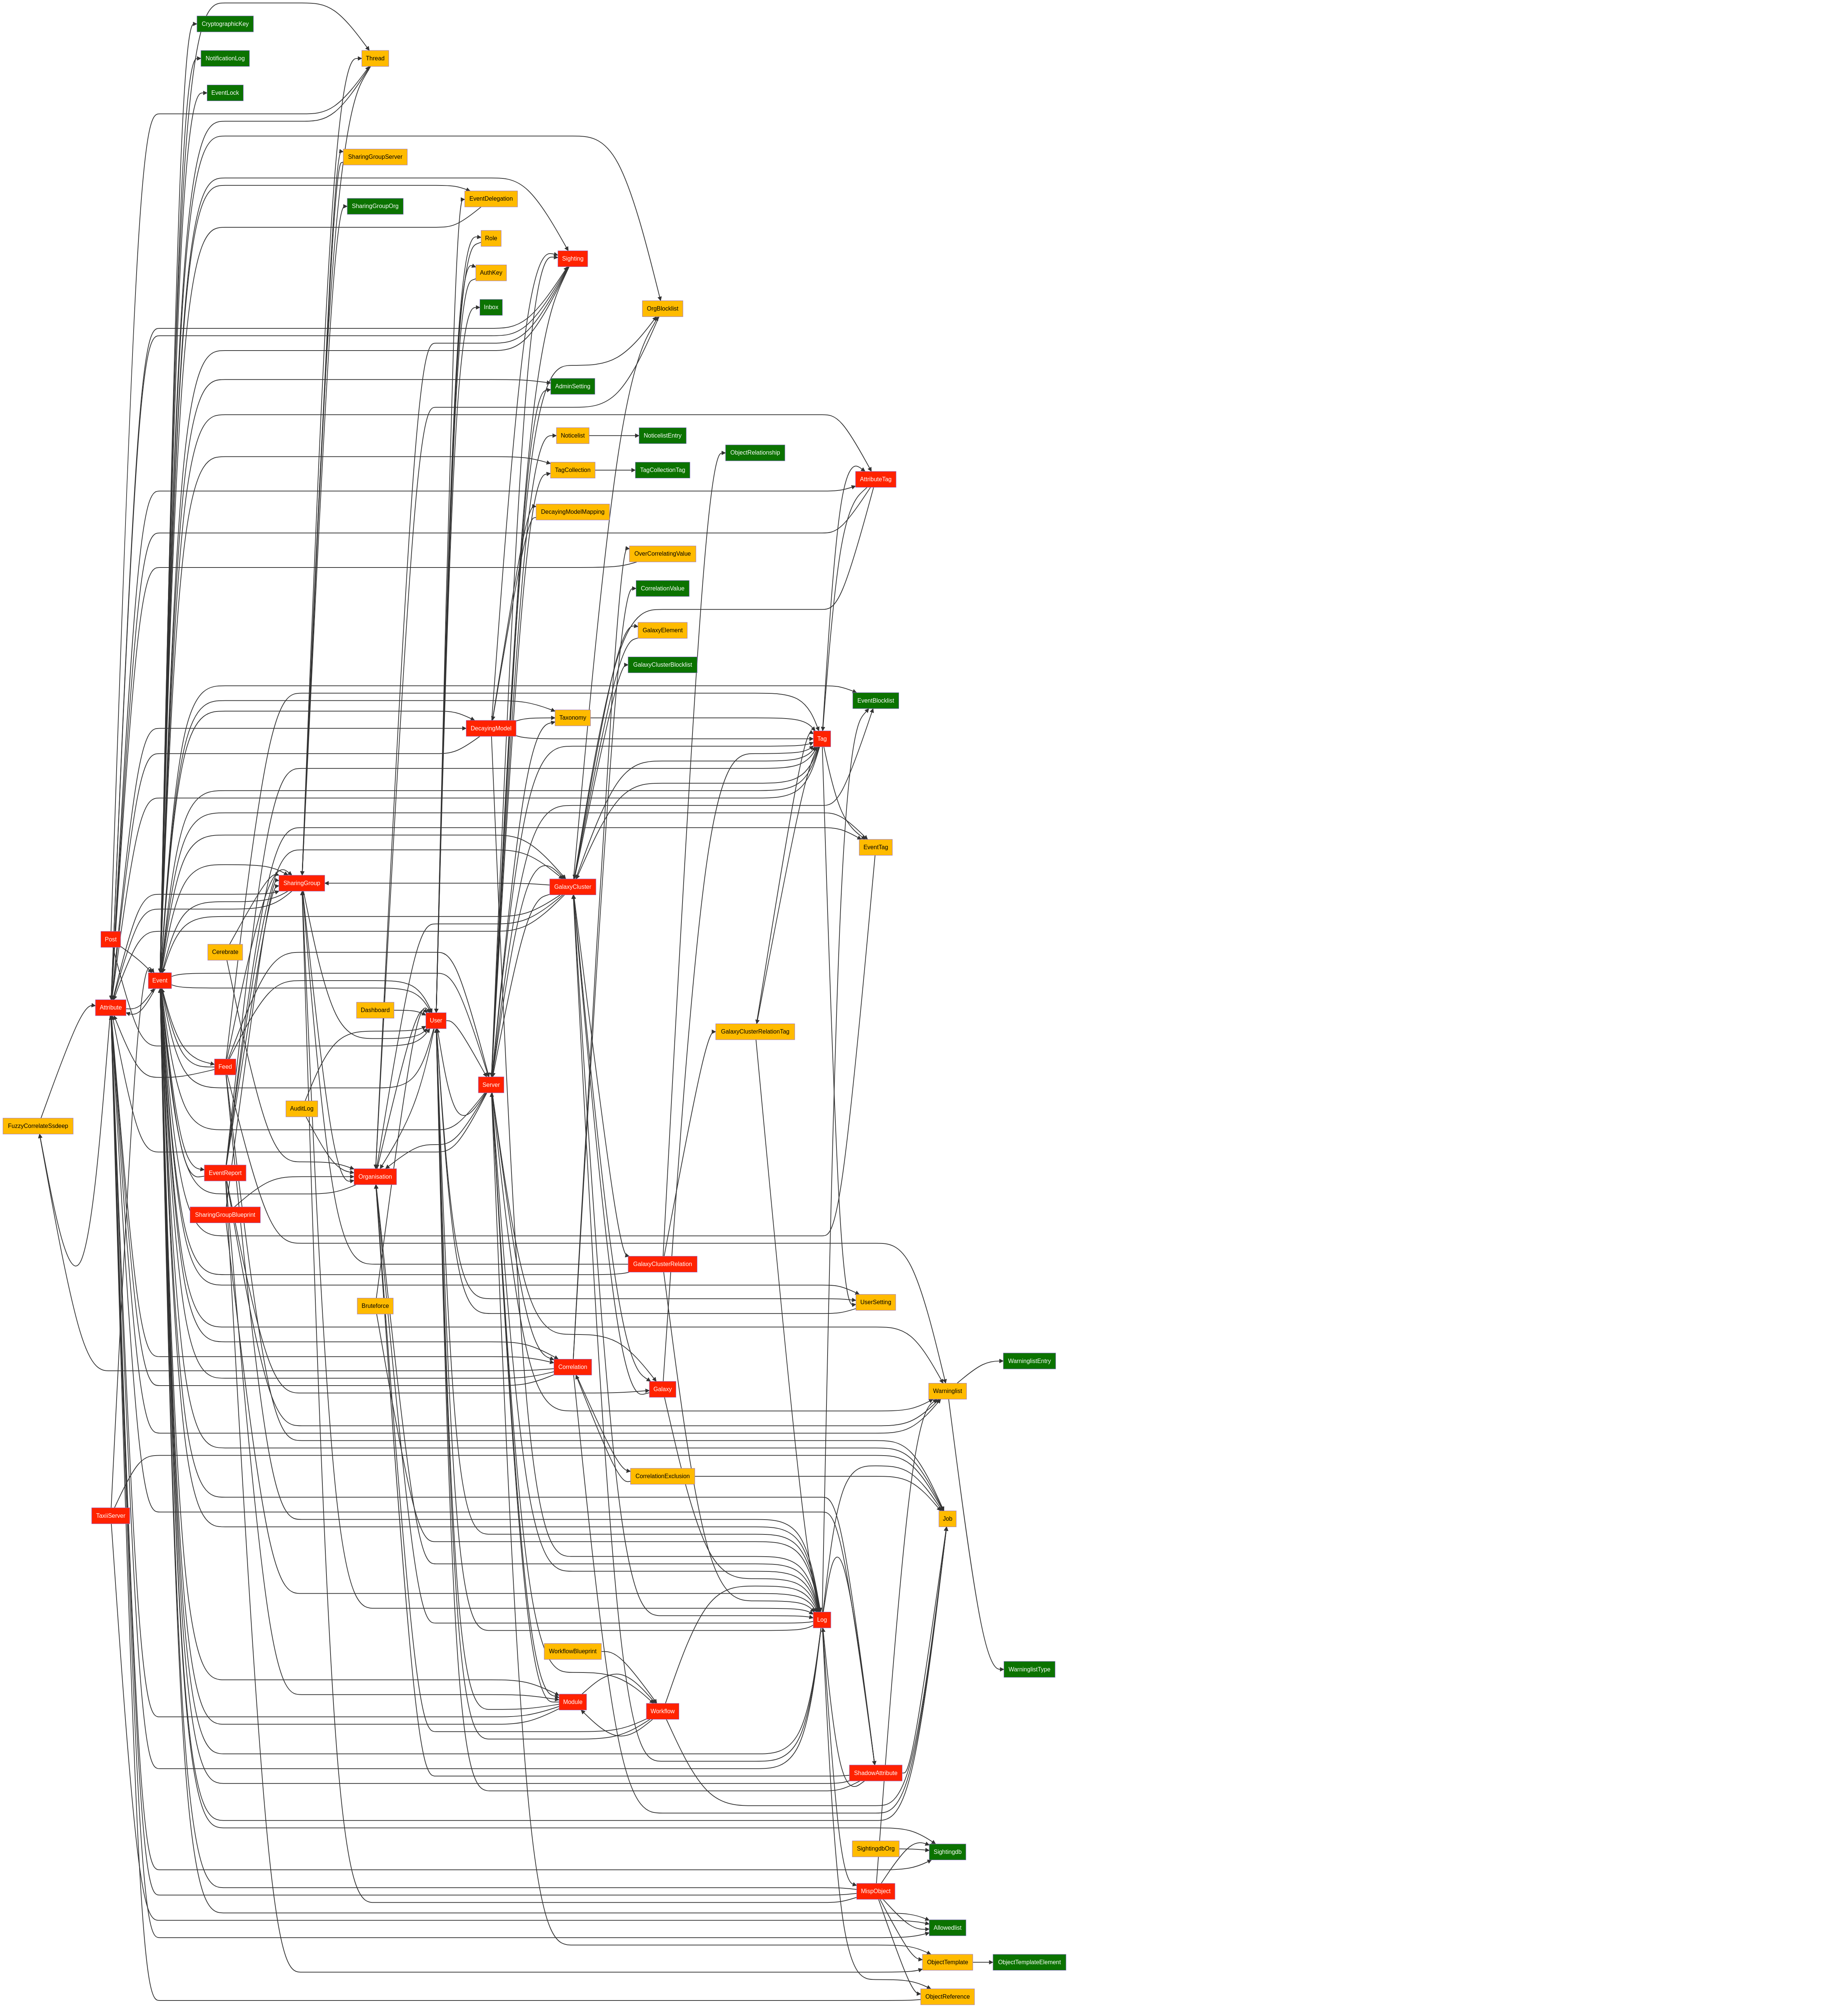
\includegraphics[scale=0.06,angle=-90,origin=c]{pictures/controller-dep.png} 
    \end{center}
\end{frame}


\section{Step II - Porting the codebase}
\begin{frame}
    \frametitle{> Step II - Roadmap for a 3-wave porting}
    \begin{center}
        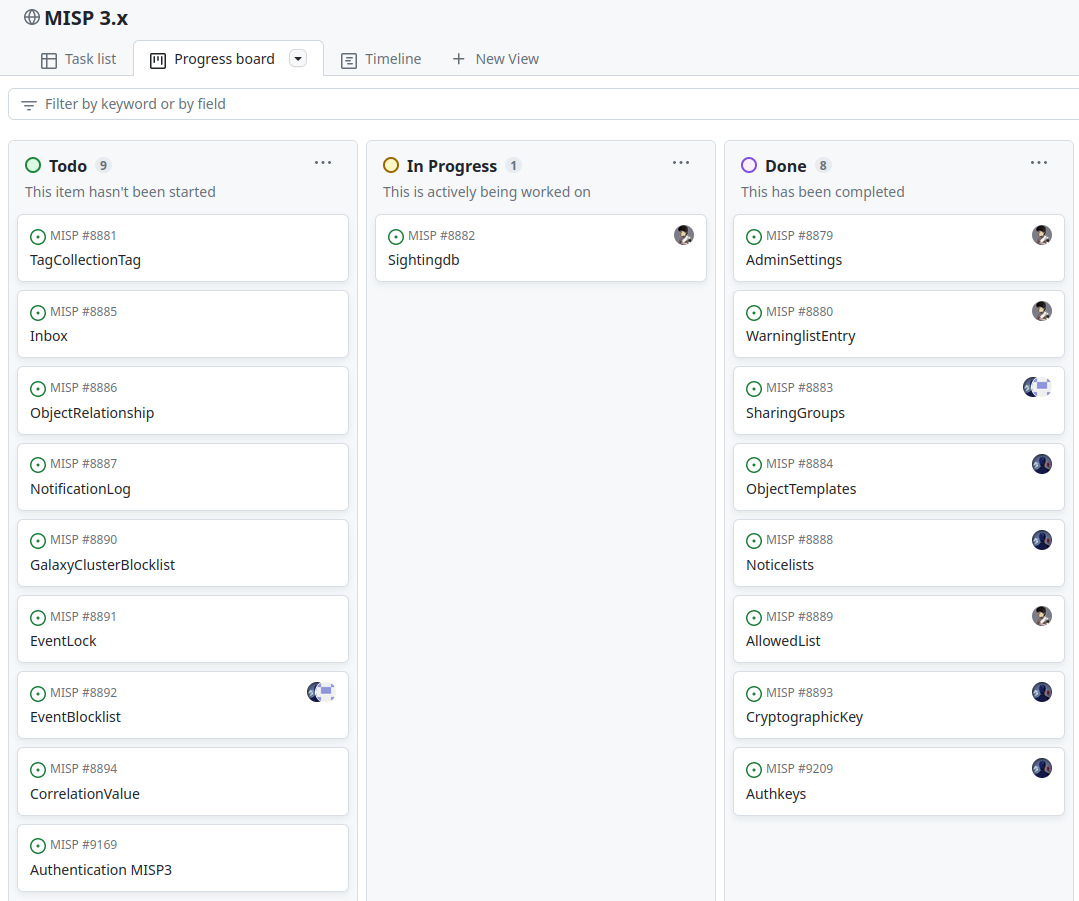
\includegraphics[width=0.99\linewidth]{pictures/misp3-github-project.png}
    \end{center}
\end{frame}

\begin{frame}
    \frametitle{> Step II - Roadmap for a 3-wave porting}
    \begin{itemize}
        \setlength\itemsep{1em}
        \item[] \textbf{\color{main}Wave 1} Least complex/inter-connected models
        \begin{itemize}
            \item E.g. Blocklist, Warninglist, Object-template, User
        \end{itemize}
        \item[] \textbf{\color{main}Wave 2} More glue relying on component already migrated
        \begin{itemize}
            \item E.g. Authkey, *-Tag, Taxonomy
        \end{itemize}
        \item[] \textbf{\color{main}Wave 3} The actual meat of the application
        \begin{itemize}
            \item E.g. Attribute, Event, Workflow
        \end{itemize}
    \end{itemize}
\end{frame}

\begin{frame}
    \frametitle{> Step II - Test driven development}
    \begin{center}
        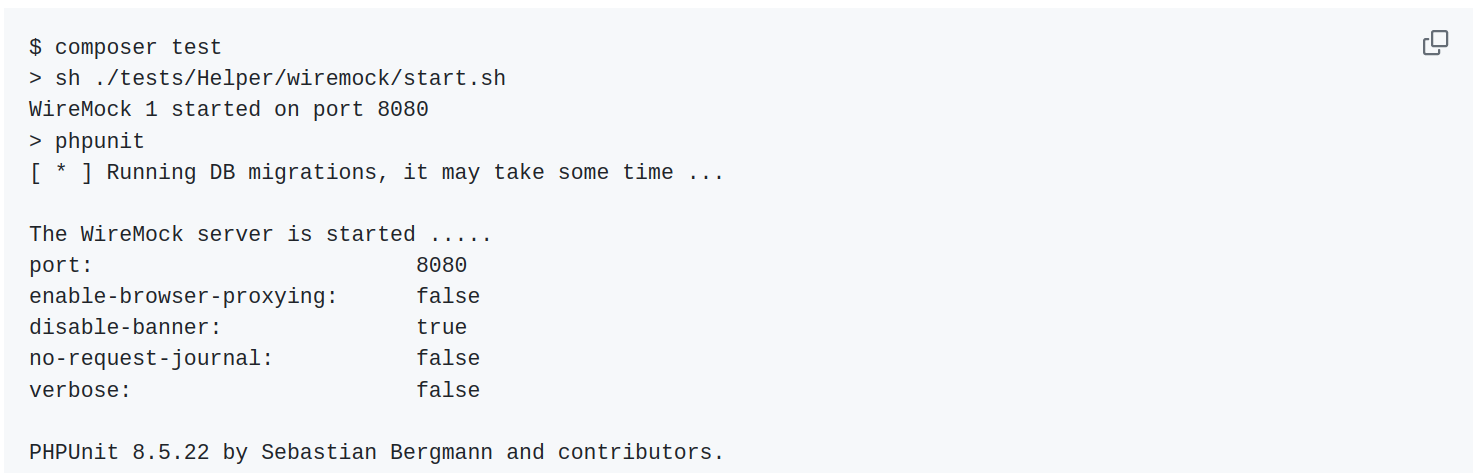
\includegraphics[width=1.0\linewidth]{pictures/phpunit.png}
    \end{center}
    \begin{itemize}
        \item Complementary to PyMISP test
        \item In-framework \textbf{Unit Tests} and \textbf{Endpoint Tests}
        \item Improved CI pipeline and enforced code standard
    \end{itemize}
\end{frame}

\begin{frame}
    \frametitle{> Codebase Migration: Where We Stand I}
    Migration officially started in January 2023
    \begin{center}
        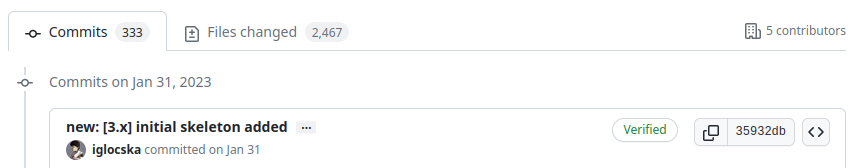
\includegraphics[width=1\linewidth]{pictures/status-2023-10-03.png}
    \end{center}
    \begin{minipage}{0.62\textwidth}
        \begin{itemize}
            \item Around \textbf{27 tables} have been moved
            \item Some partially, others completely
        \end{itemize}
    \end{minipage}%
    \begin{minipage}{0.33\textwidth}
        \;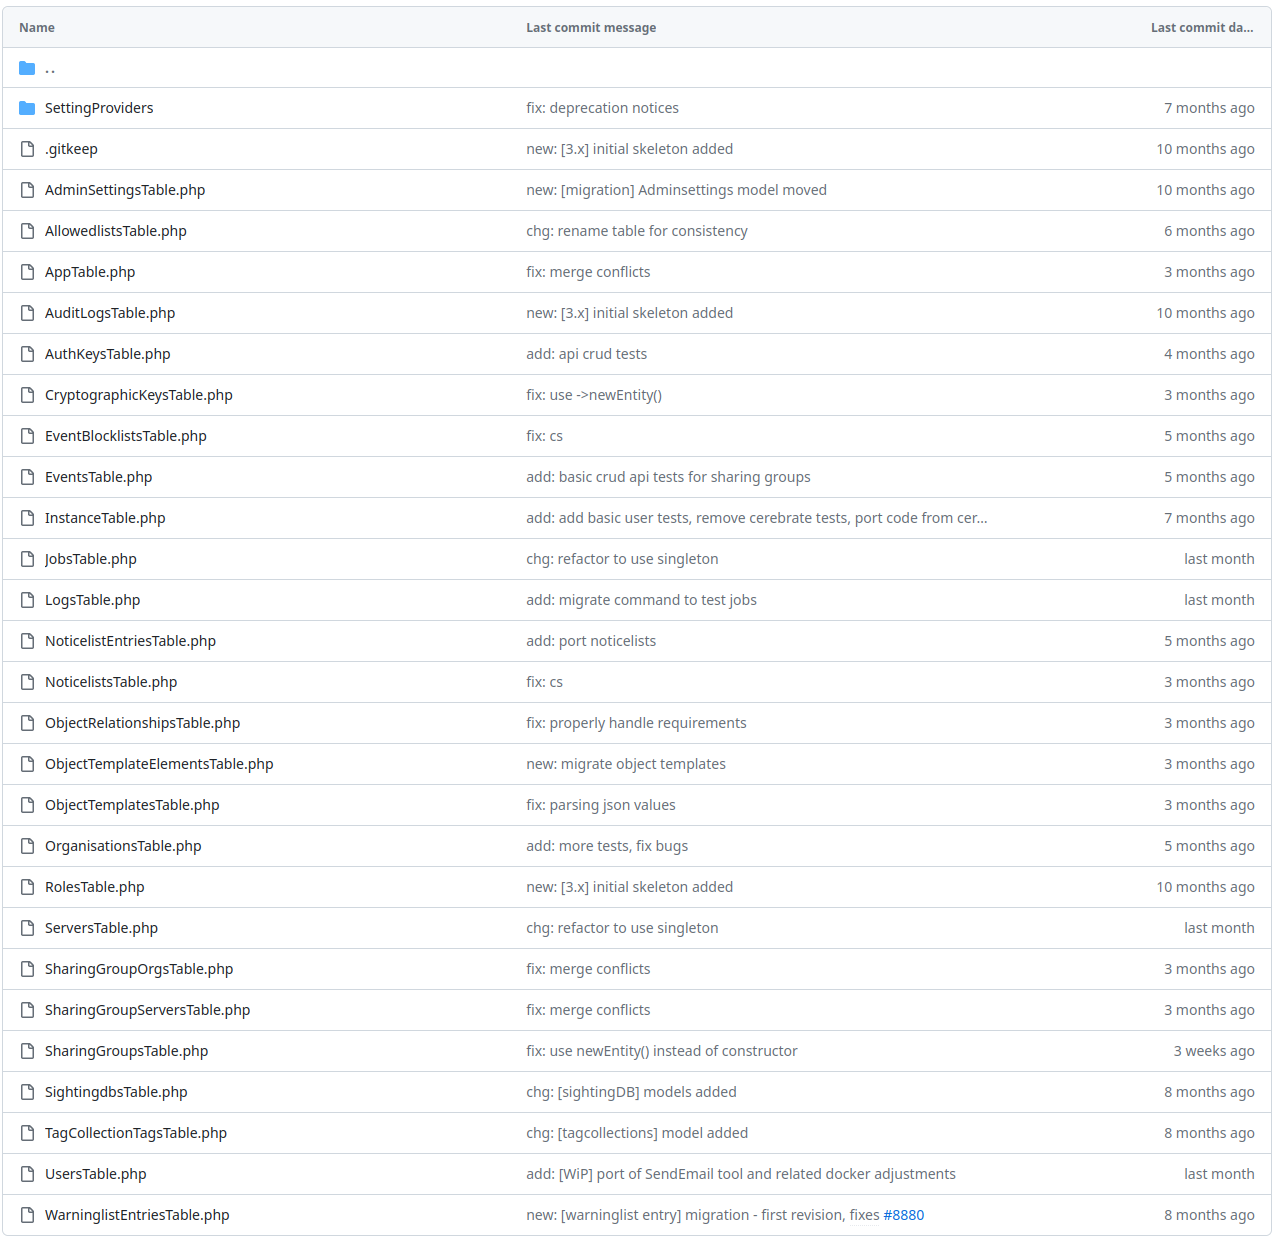
\includegraphics[width=1.2\linewidth]{pictures/migrated-models.png}
    \end{minipage}
    
\end{frame}

\begin{frame}
    \frametitle{> Codebase Migration: Where We Stand II}
    \begin{center}
        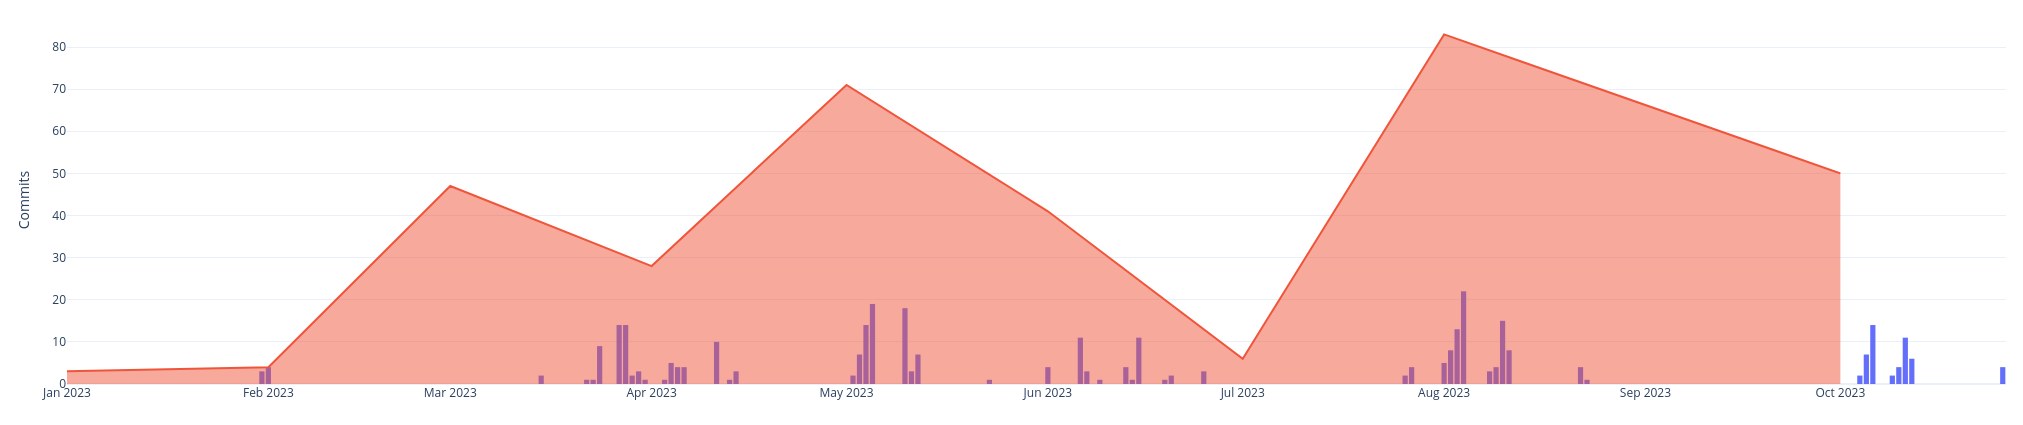
\includegraphics[width=1\linewidth]{pictures/ramping-up.png}
    \end{center}
    \begin{itemize}
        \item Migration speed ramping up. The more we port, the faster we go
    \end{itemize}
    \begin{center}
        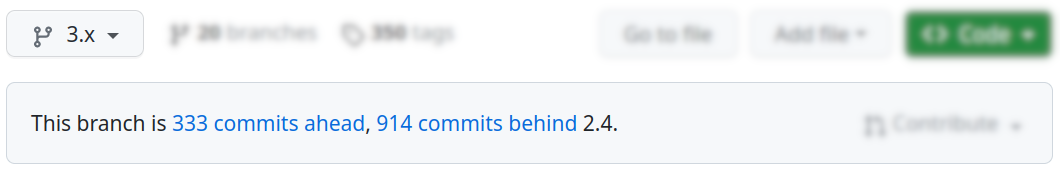
\includegraphics[width=1\linewidth]{pictures/catering-to-2.4.png}
    \end{center}
    \begin{itemize}
        \item Even while supporting and improving \texttt{2.4}
    \end{itemize}
\end{frame}

\section{Look and Feel}
\begin{frame}
    \frametitle{Codebase Migration: Look and Feel I}
    \begin{itemize}
        \item Most of the changes are \textbf{invisible}
        \item Some user interfaces can still be displayed
    \end{itemize}
    \begin{center}
        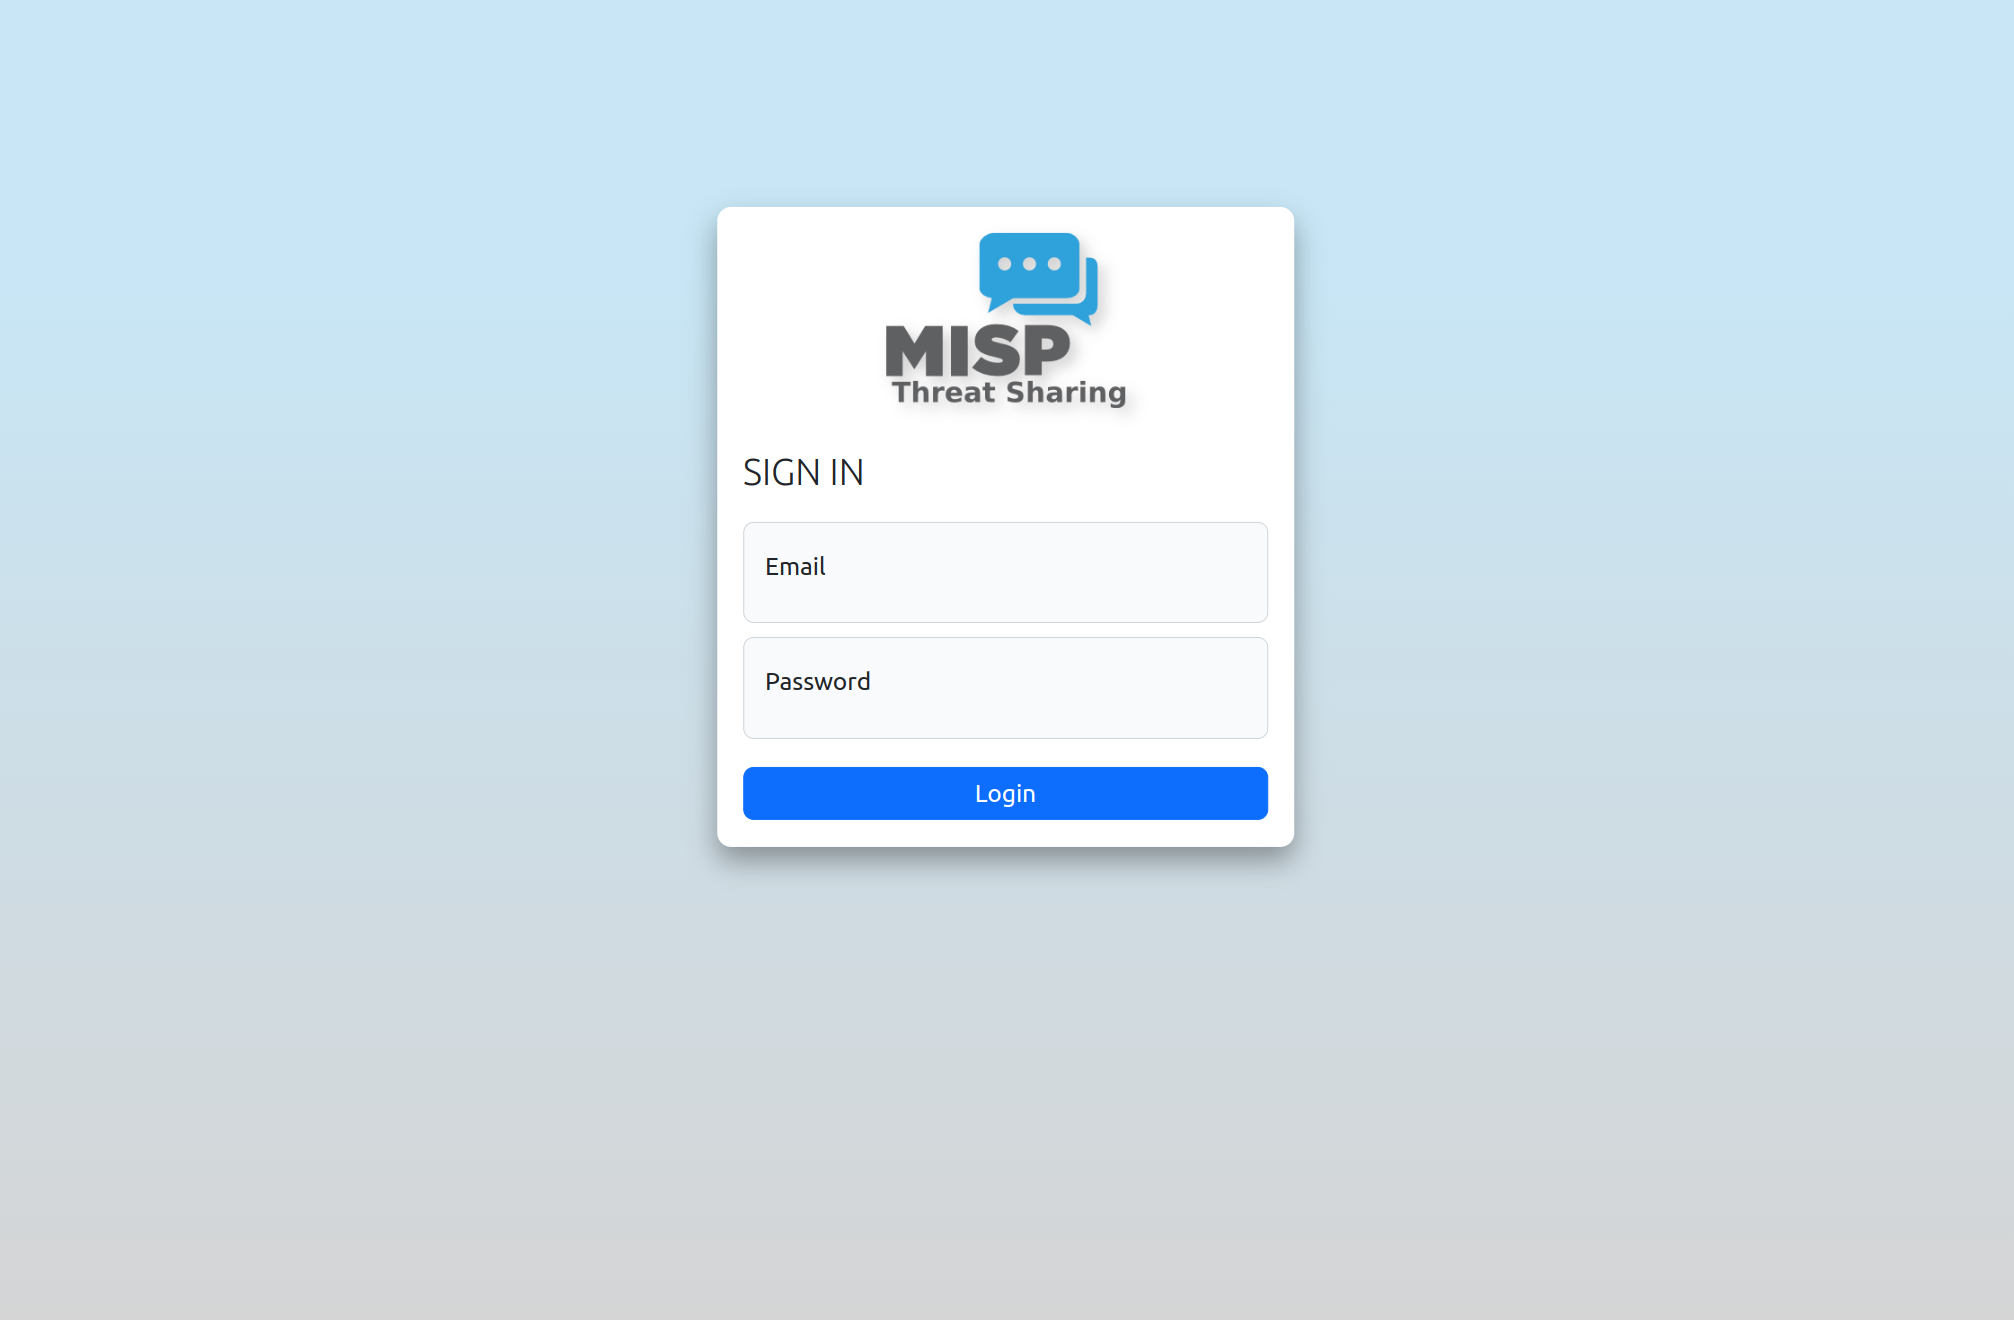
\includegraphics[width=0.8\linewidth]{pictures/login-screen.png}
    \end{center}
\end{frame}

\begin{frame}
    \frametitle{Codebase Migration: Look and Feel II}
    \begin{center}
        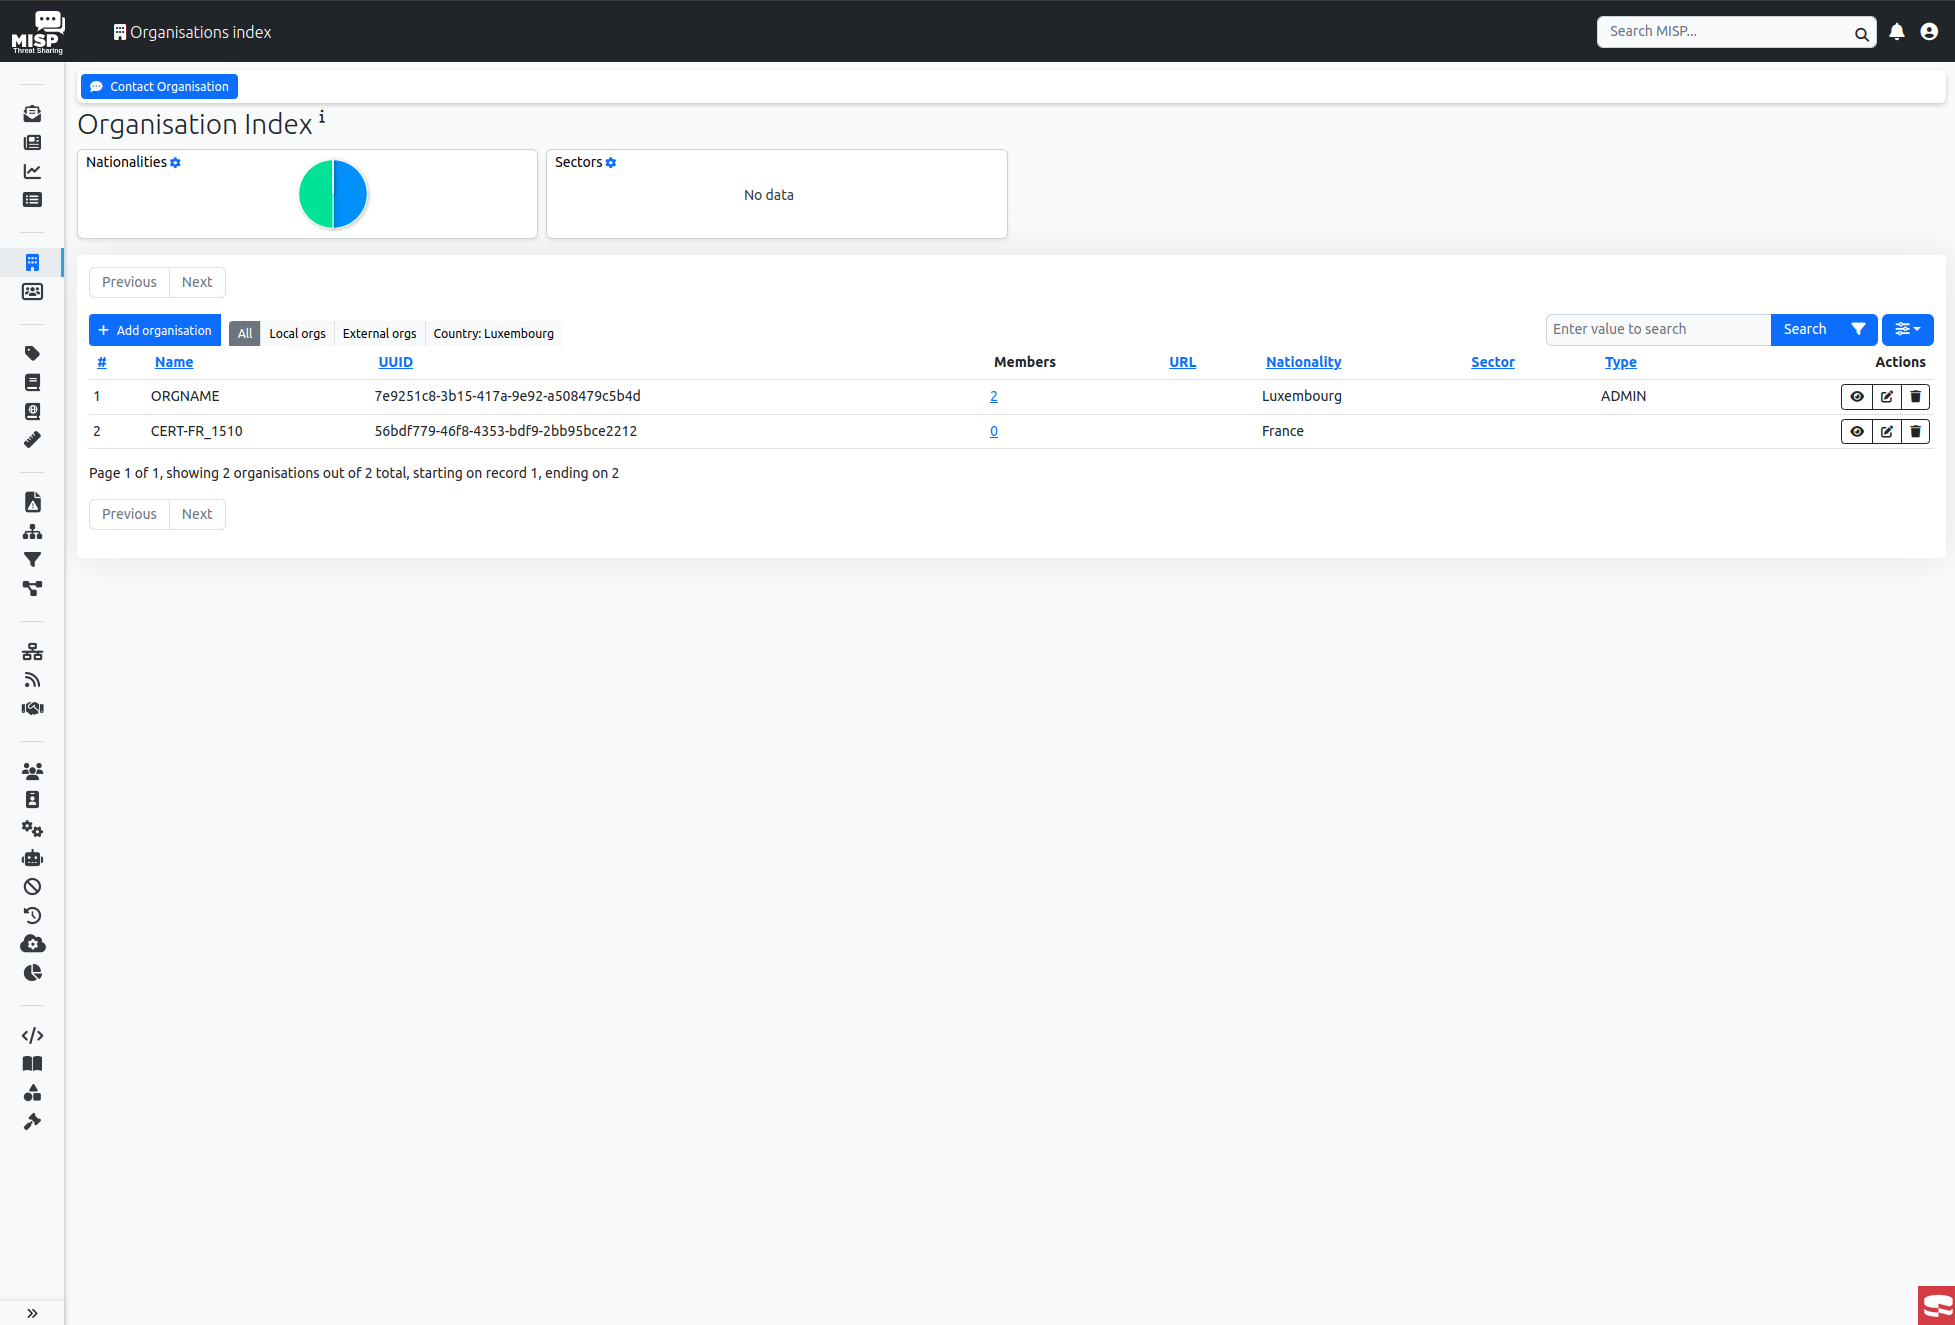
\includegraphics[width=1.0\linewidth]{pictures/organisation-index.png}
    \end{center}
\end{frame}

\begin{frame}
    \frametitle{Codebase Migration: Look and Feel II}
    \begin{center}
        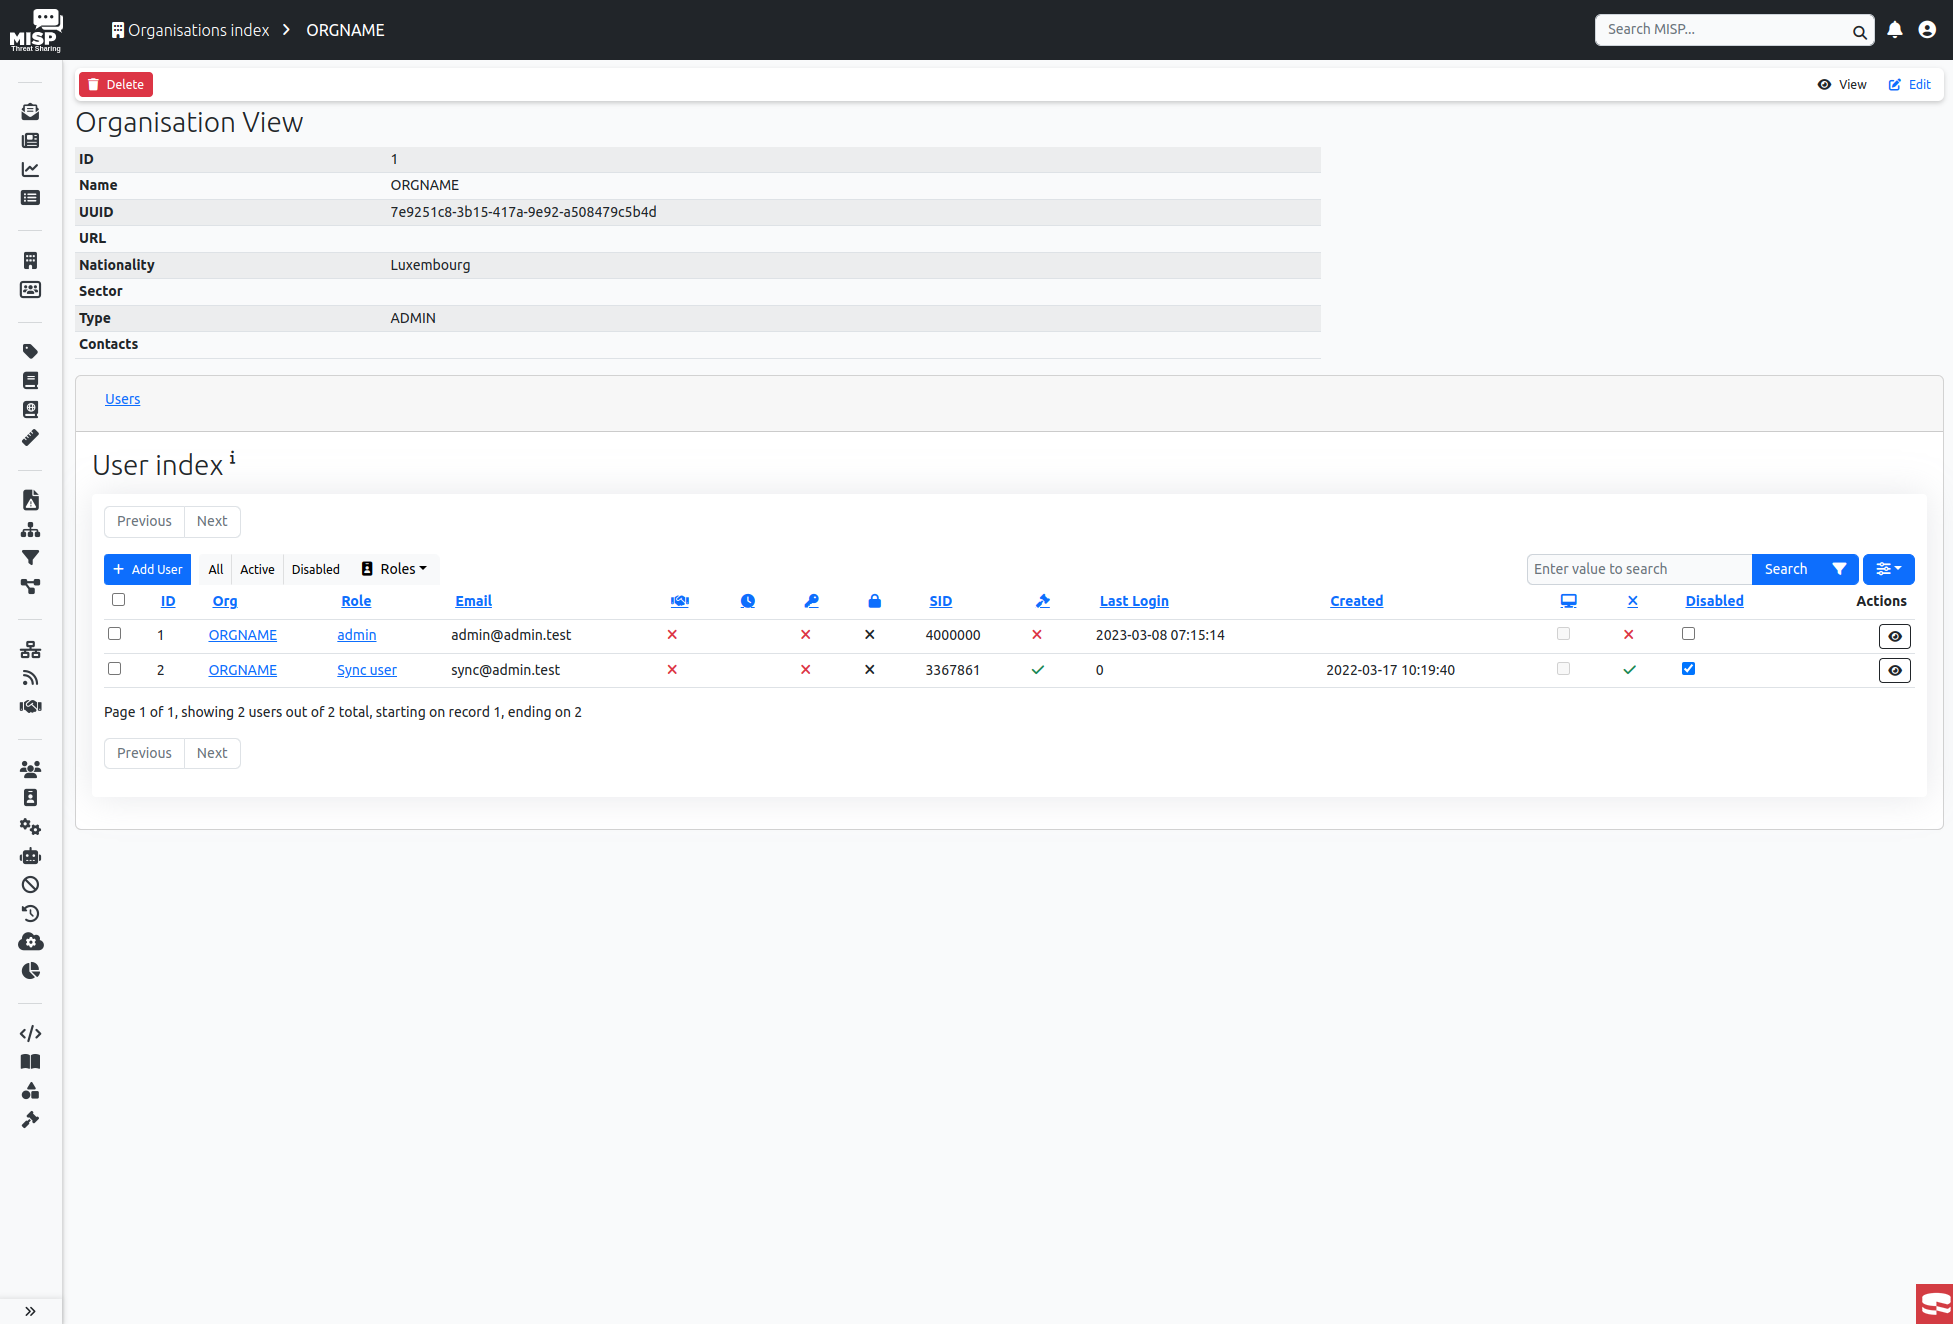
\includegraphics[width=1.0\linewidth]{pictures/organisation-view.png}
    \end{center}
\end{frame}

\begin{frame}
    \frametitle{Codebase Migration: Look and Feel II}
    \begin{center}
        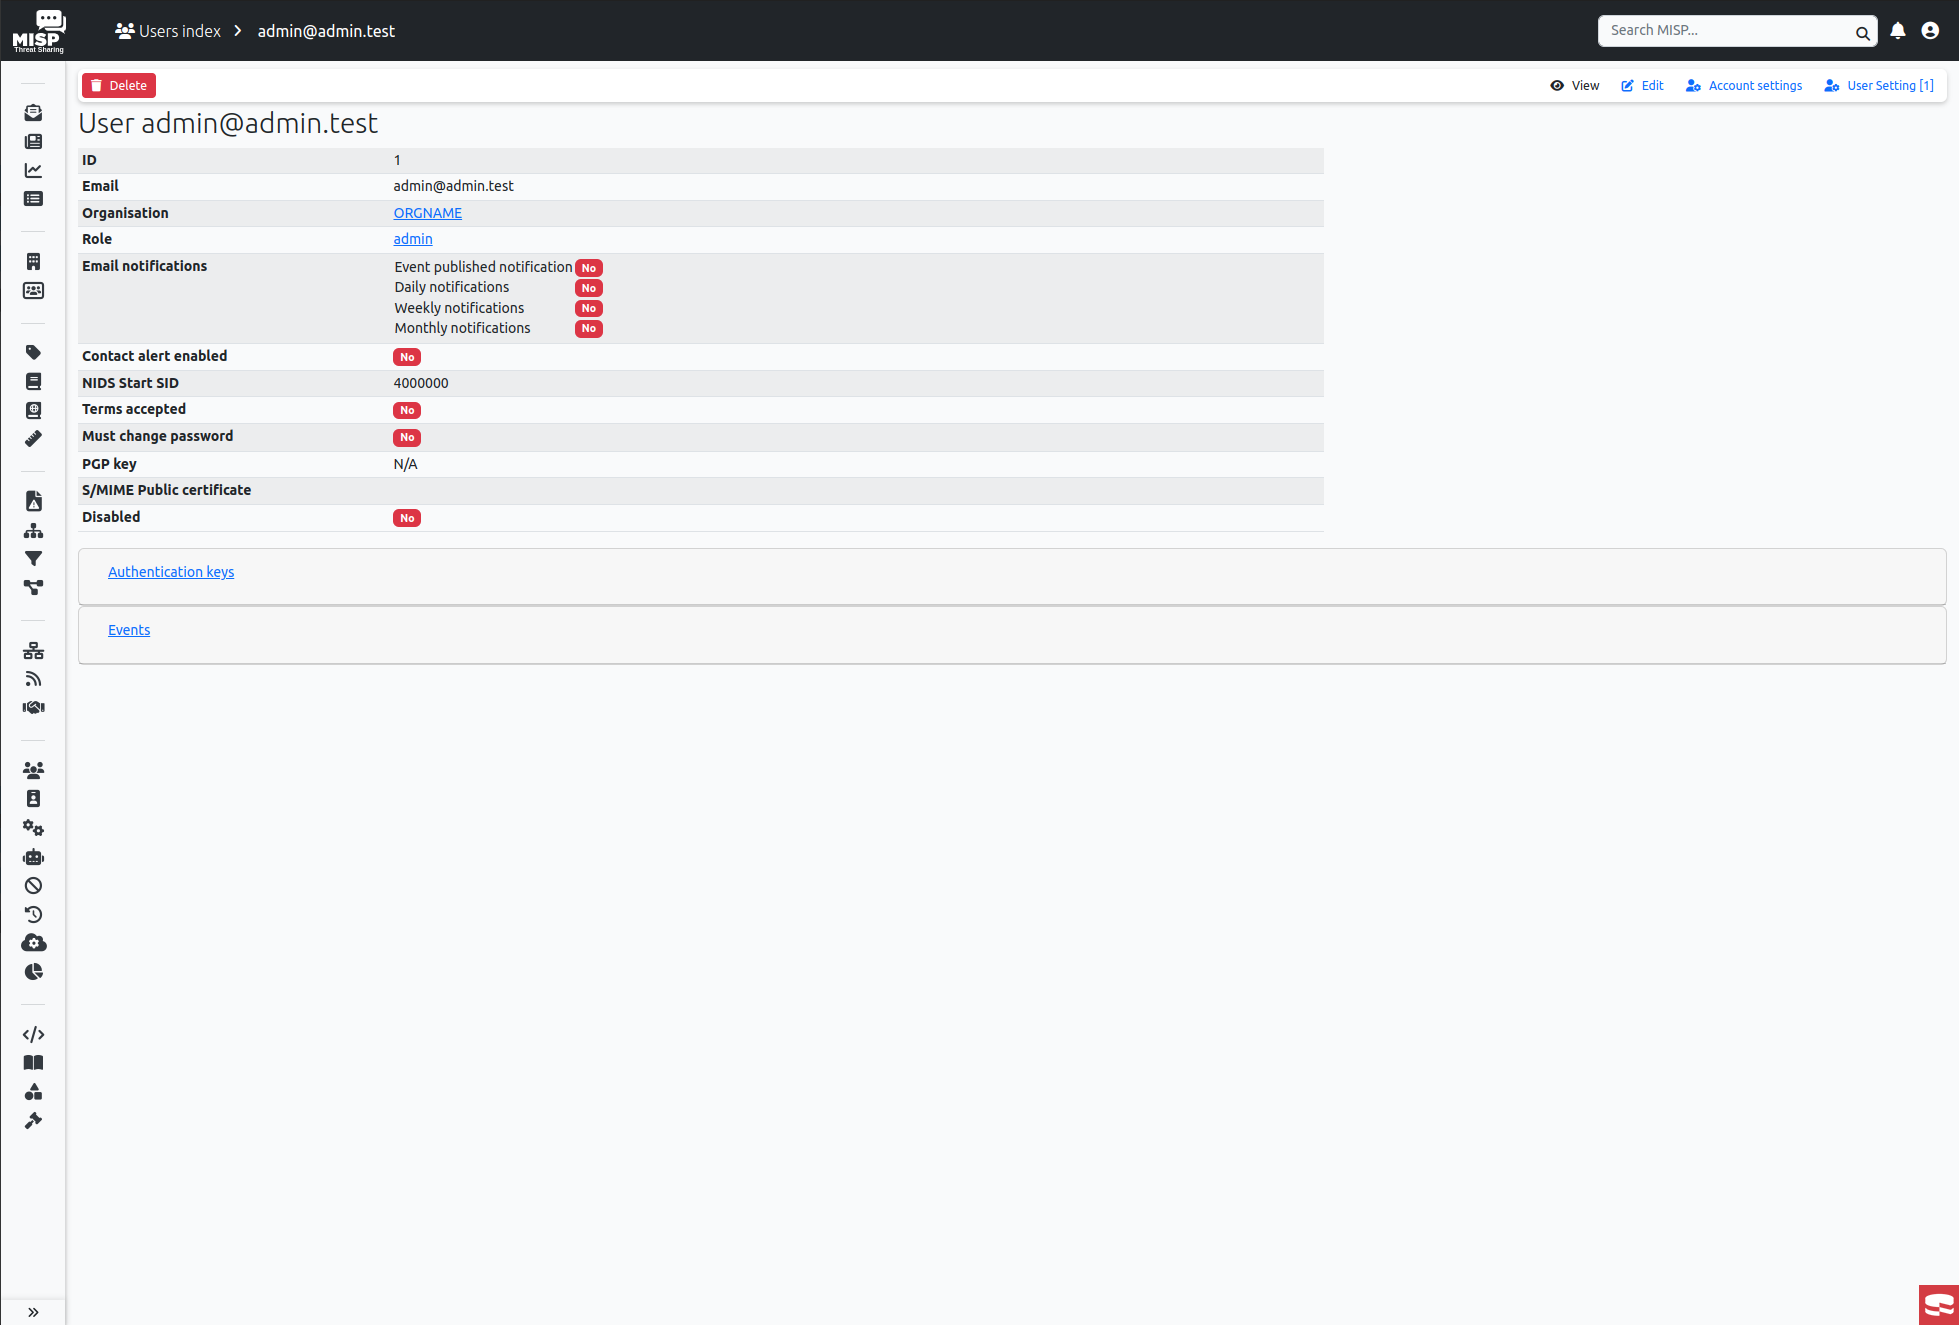
\includegraphics[width=1.0\linewidth]{pictures/user-view.png}
    \end{center}
\end{frame}

\begin{frame}
    \frametitle{Codebase Migration: Look and Feel II}
    \begin{center}
        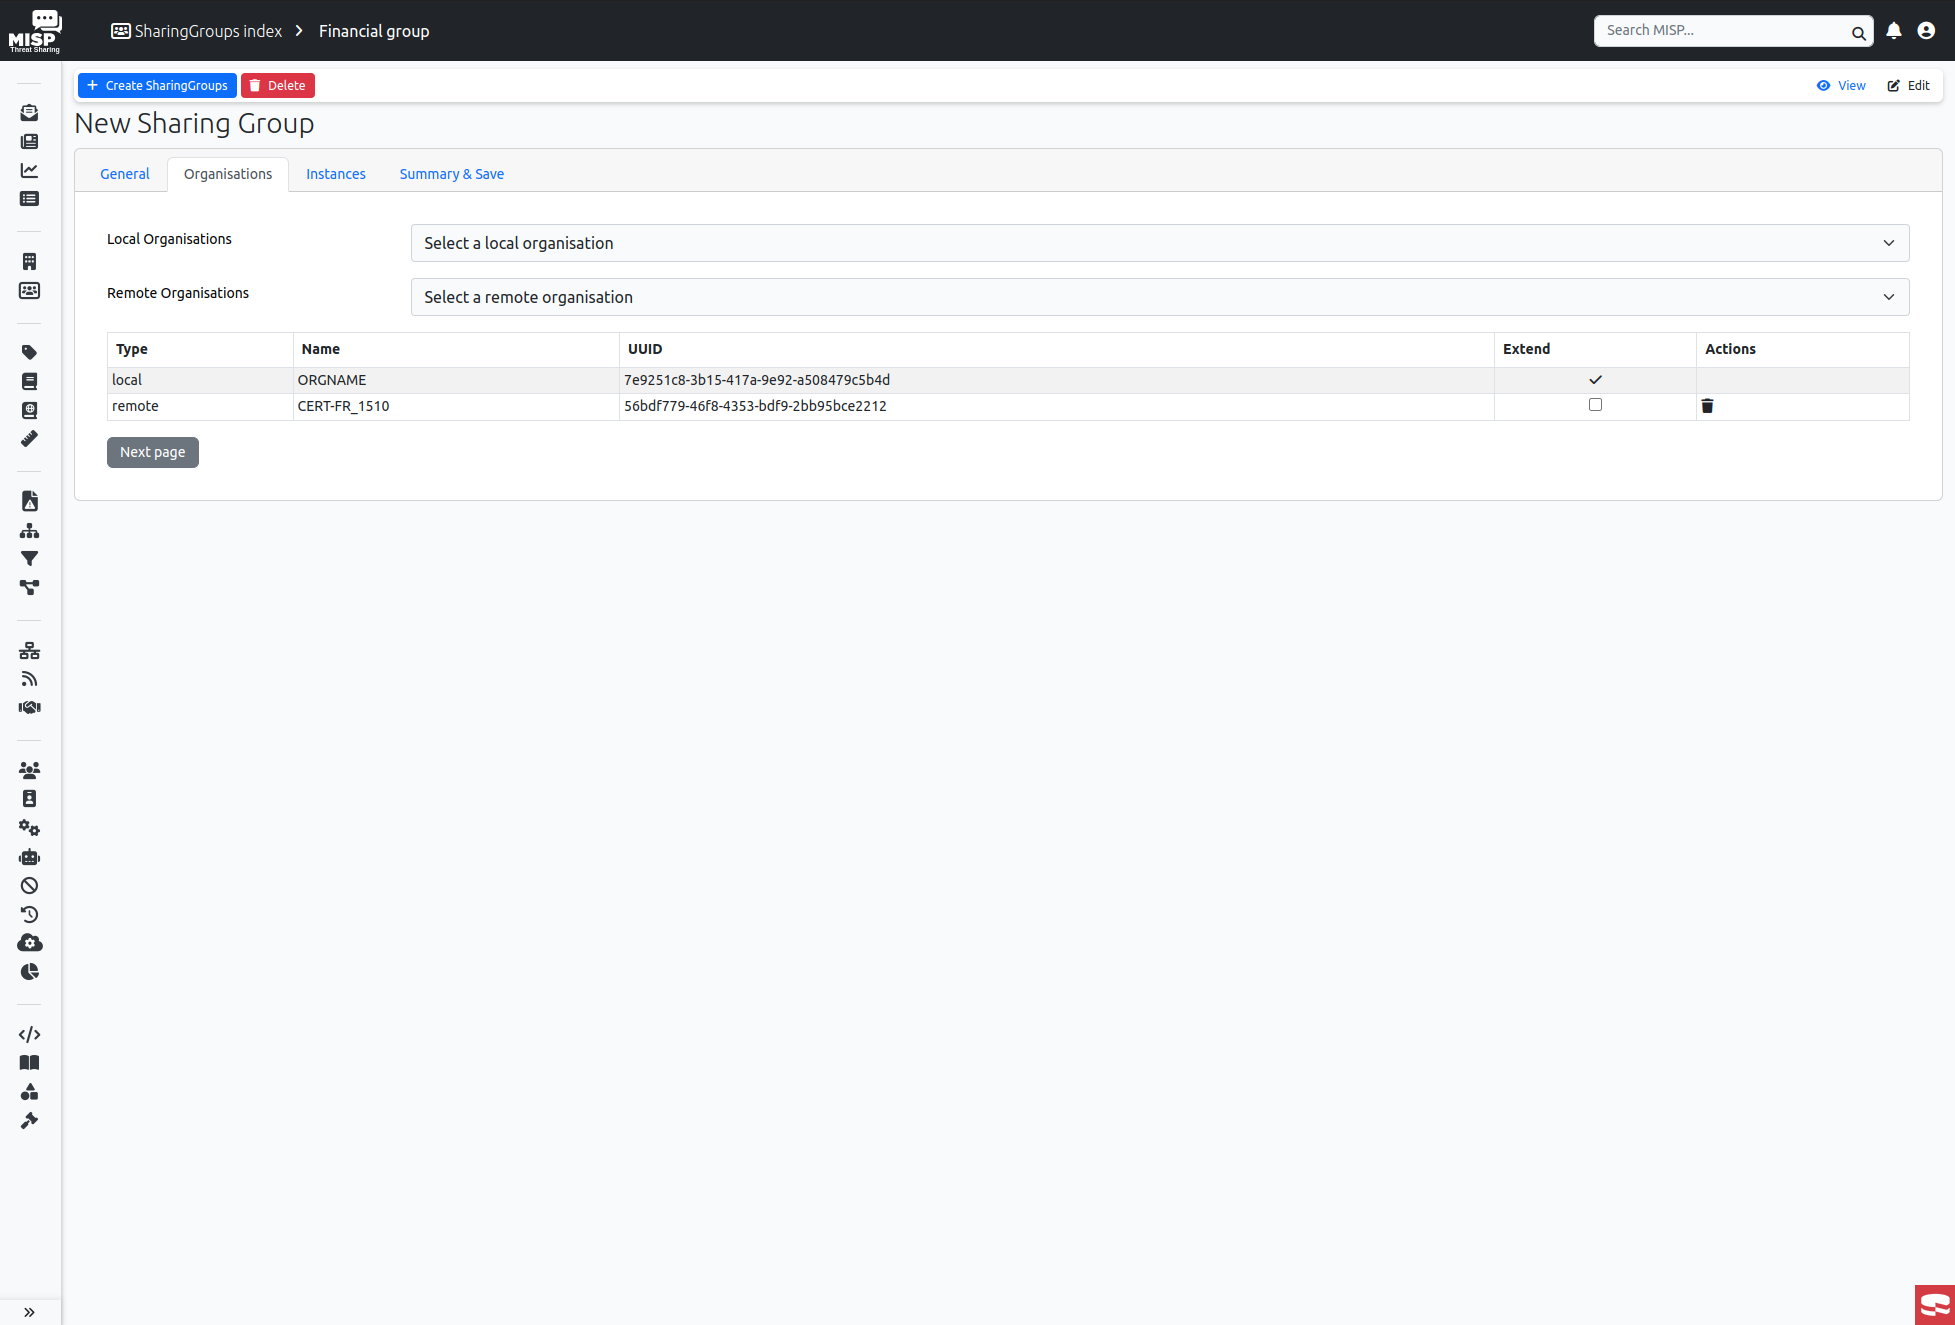
\includegraphics[width=1.0\linewidth]{pictures/sharinggroup-add.png}
    \end{center}
\end{frame}

\begin{frame}
    \frametitle{Codebase Migration: Look and Feel II}
    \begin{minipage}{0.6\textwidth}
        \begin{itemize}
            \item Updating Bootstrap greatly improves aesthetics
            \item And allow us to integrate themes seamlessly
        \end{itemize}
    \end{minipage}%
    \begin{minipage}{0.4\textwidth}
        \begin{center}
            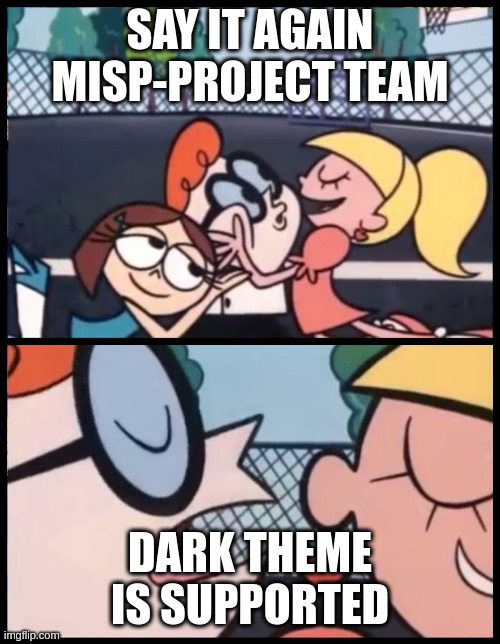
\includegraphics[width=0.9\linewidth]{pictures/dark-theme-meme.jpg}
        \end{center}
    \end{minipage}
\end{frame}

\begin{frame}
    \frametitle{Codebase Migration: Look and Feel II}
    \begin{minipage}{0.5\textwidth}
        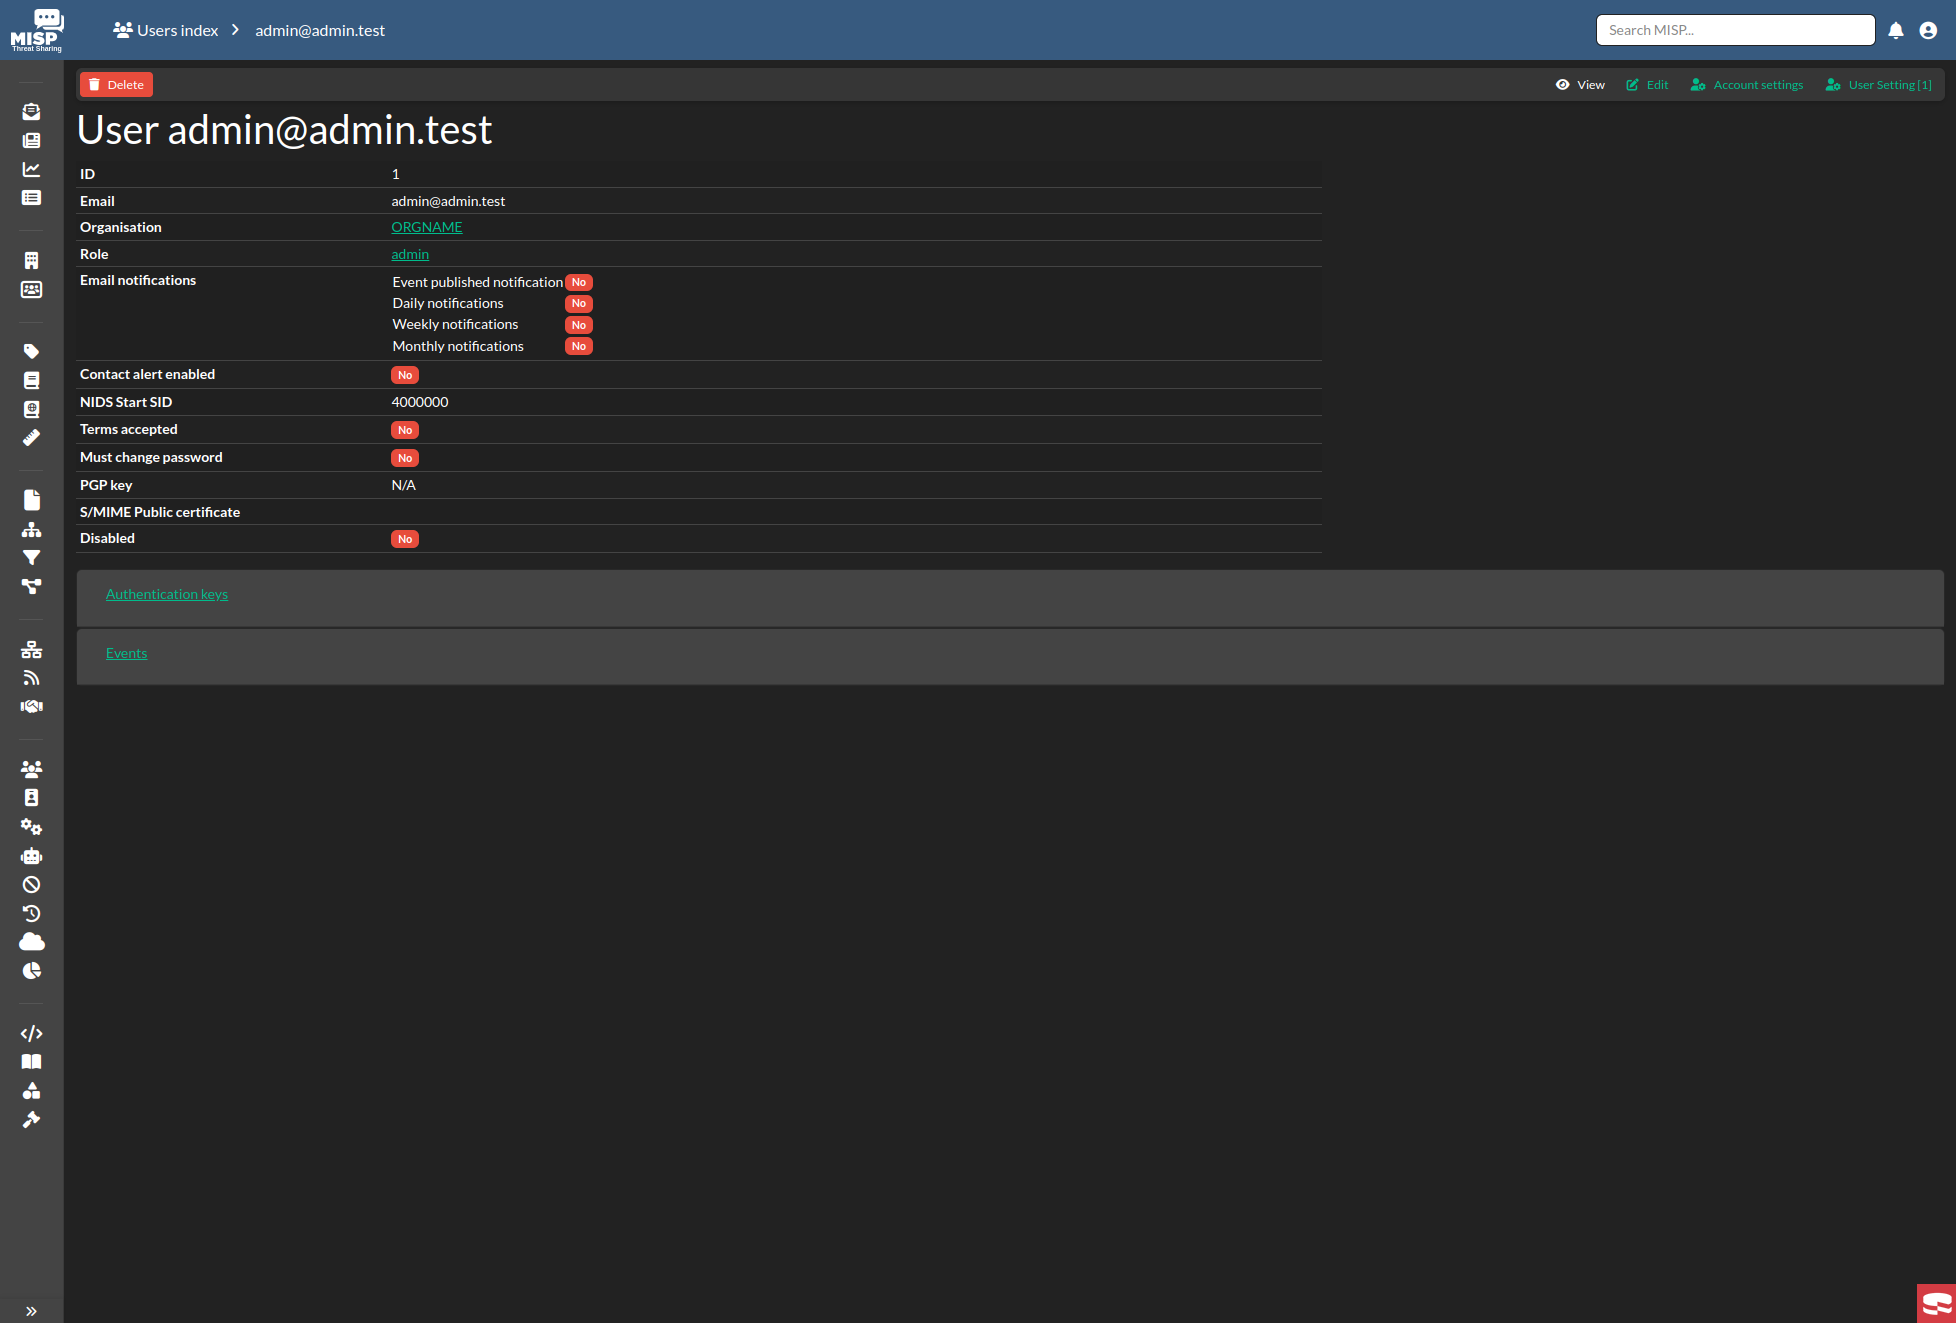
\includegraphics[width=0.9\linewidth]{pictures/theme1.png}
        \vspace{1em}
        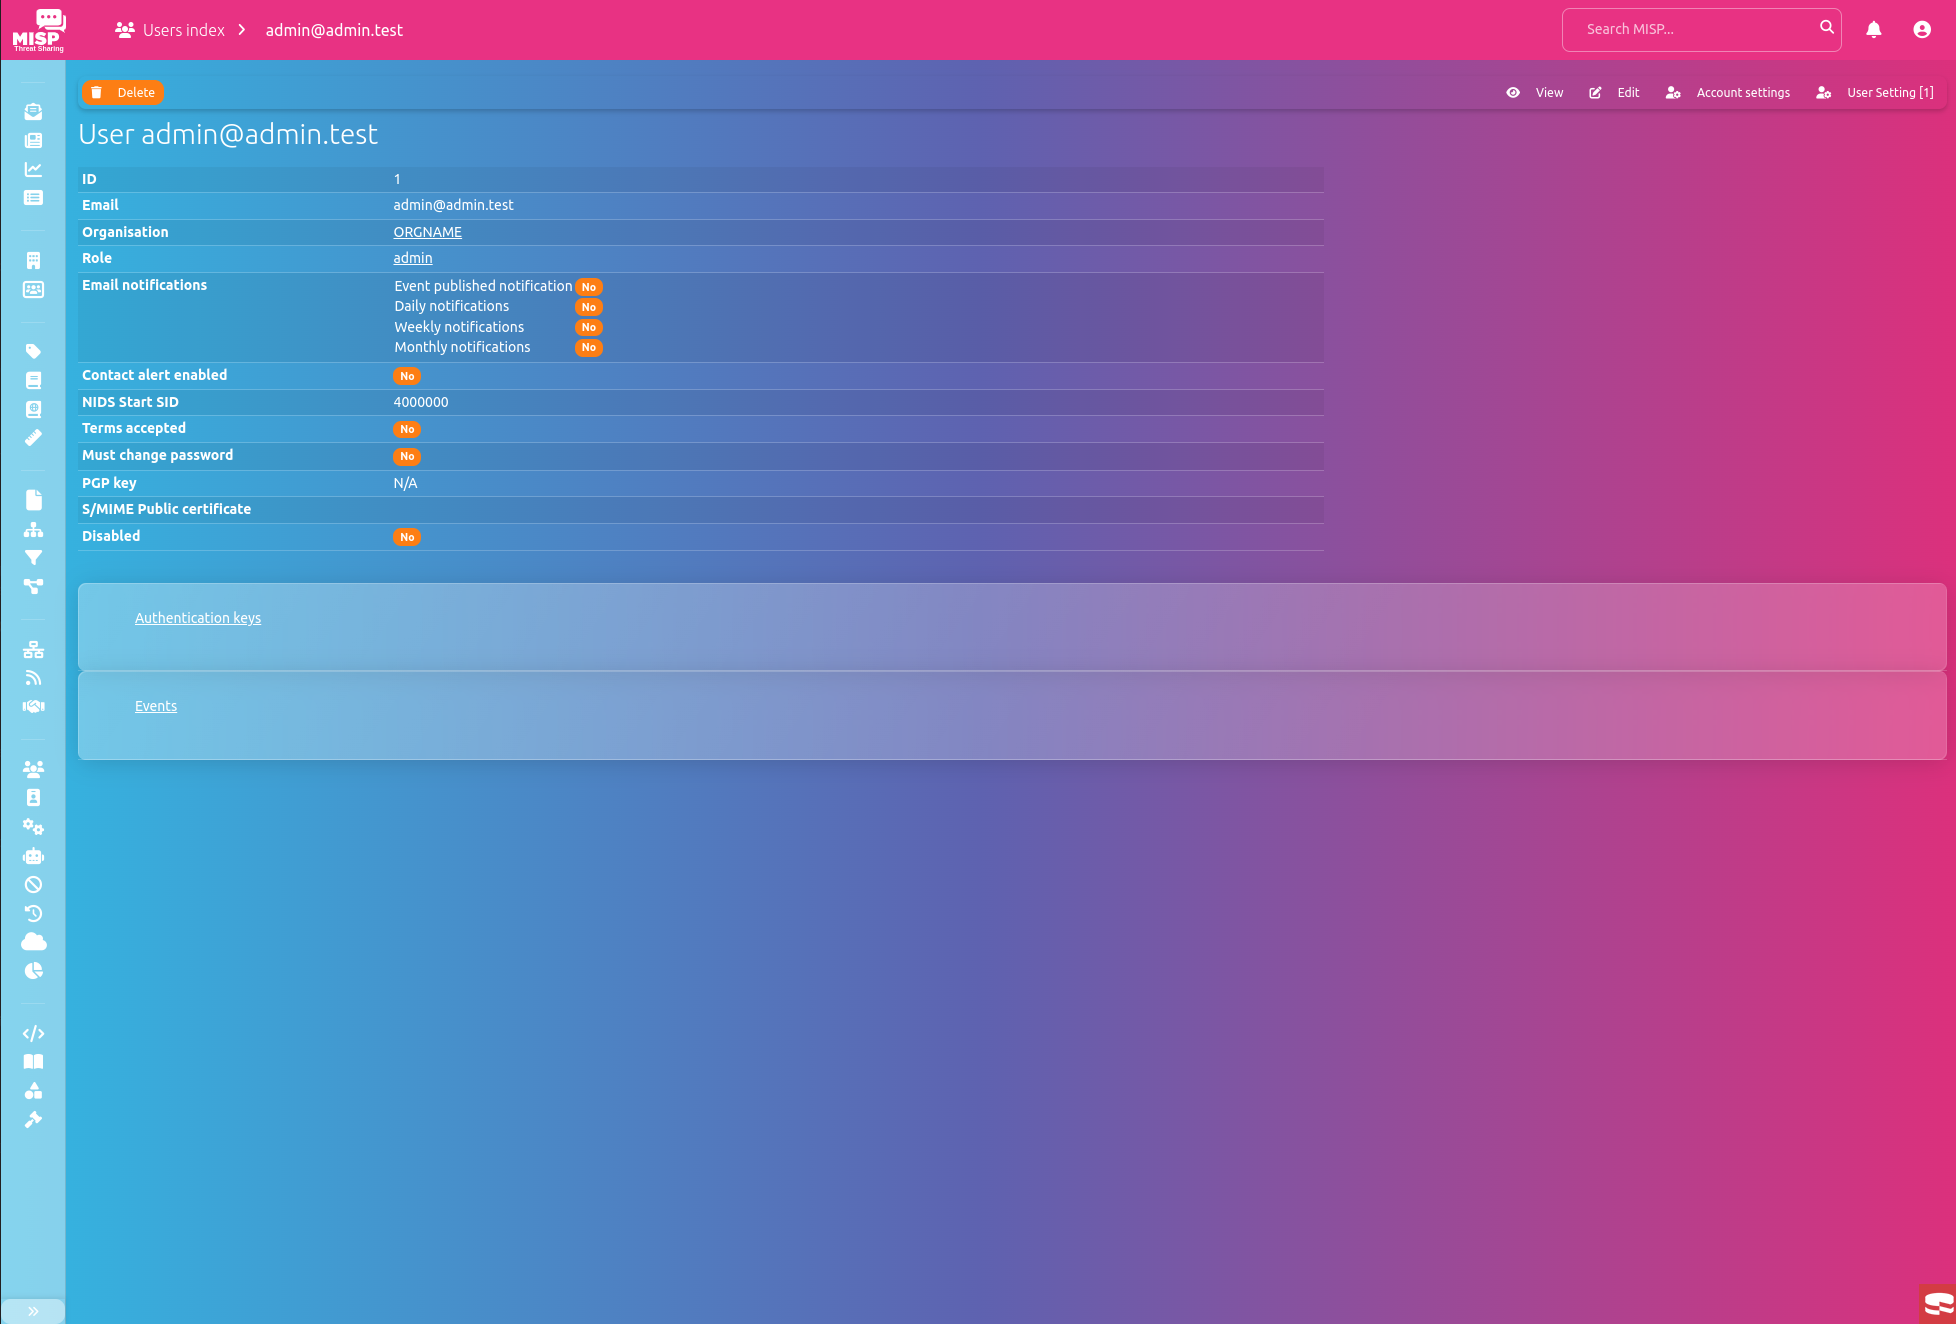
\includegraphics[width=0.9\linewidth]{pictures/theme2.png}
    \end{minipage}%
    \begin{minipage}{0.5\textwidth}
        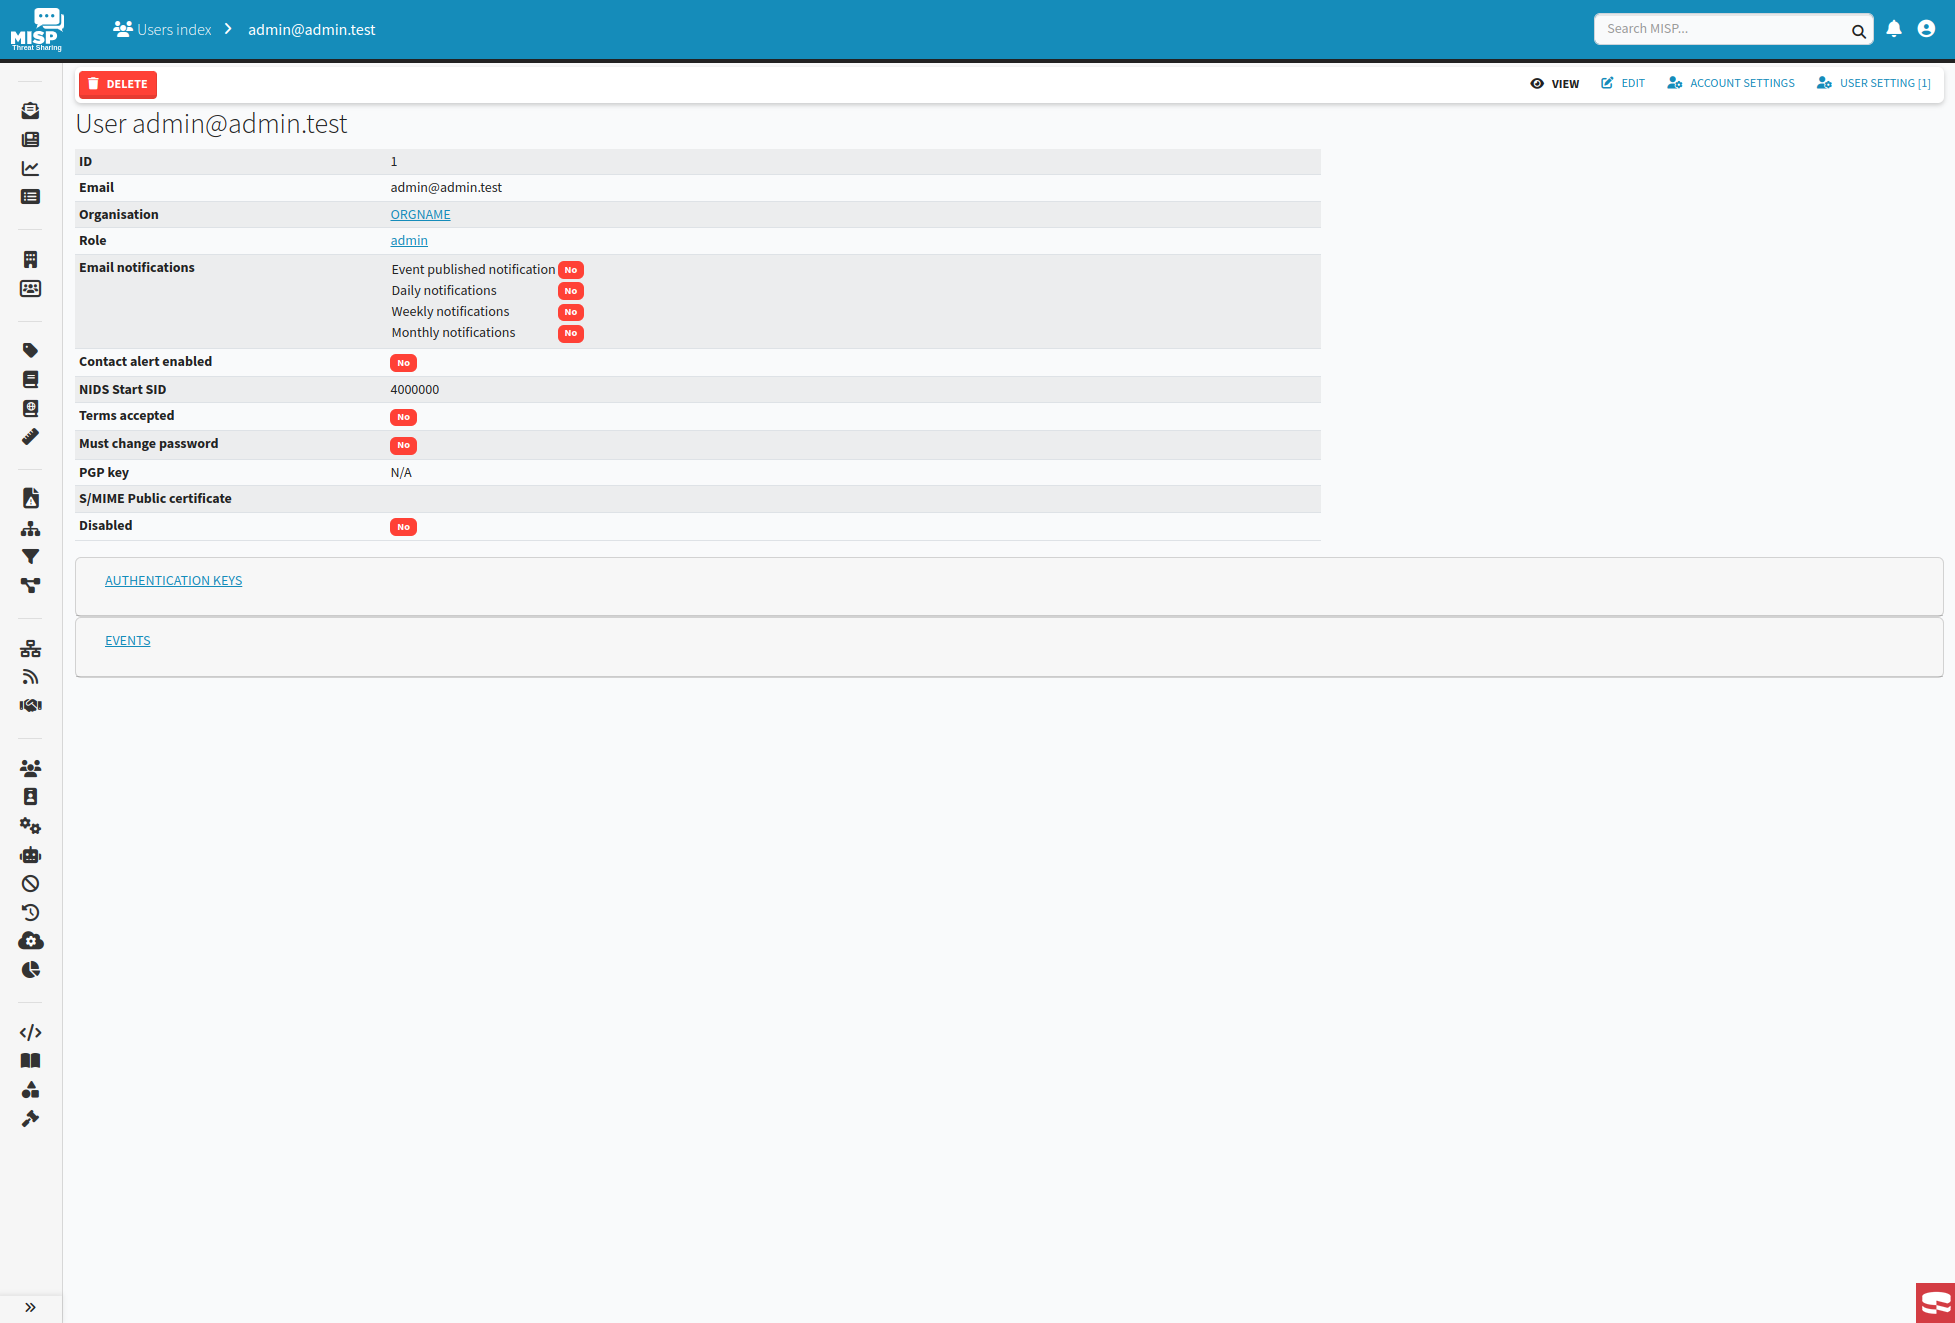
\includegraphics[width=0.9\linewidth]{pictures/theme3.png}
        \vspace{1em}
        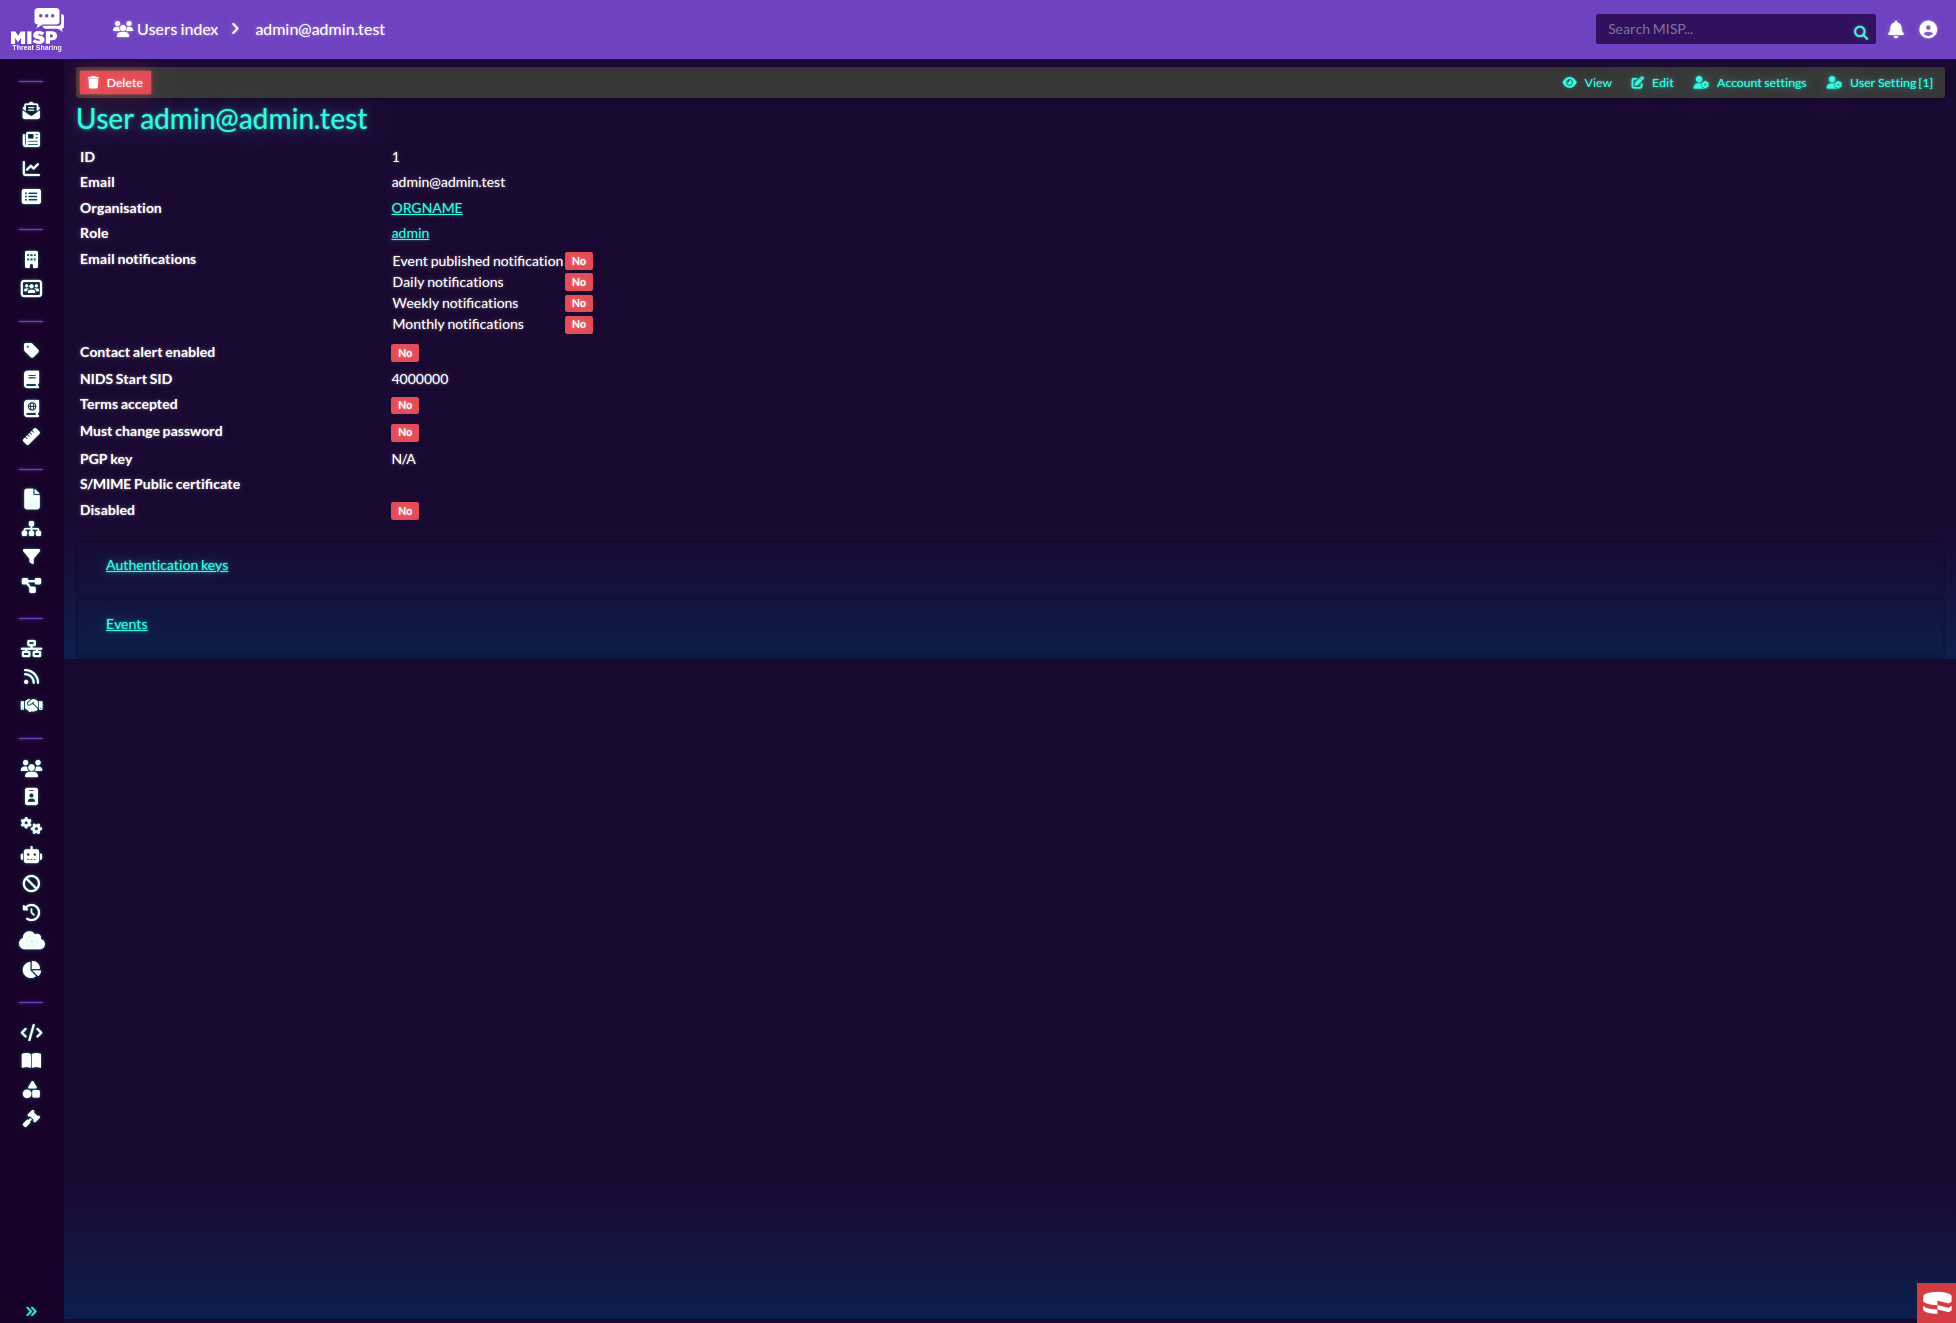
\includegraphics[width=0.9\linewidth]{pictures/theme4.png}
    \end{minipage}
\end{frame}


\section{Step III - The TODOs}
\begin{frame}
    \frametitle{> Redefine how we interact with data I}
    \begin{itemize}
        \item Indicator centric perspective
        \begin{itemize}
            \item Unified view of everything we know about a given Indicator
            \item Allows us to take better decisions
            \item Enable users to manage their IoC working set
            \item Start an investigation more easily from a single indicator
        \end{itemize}
    \end{itemize}
    \begin{center}
        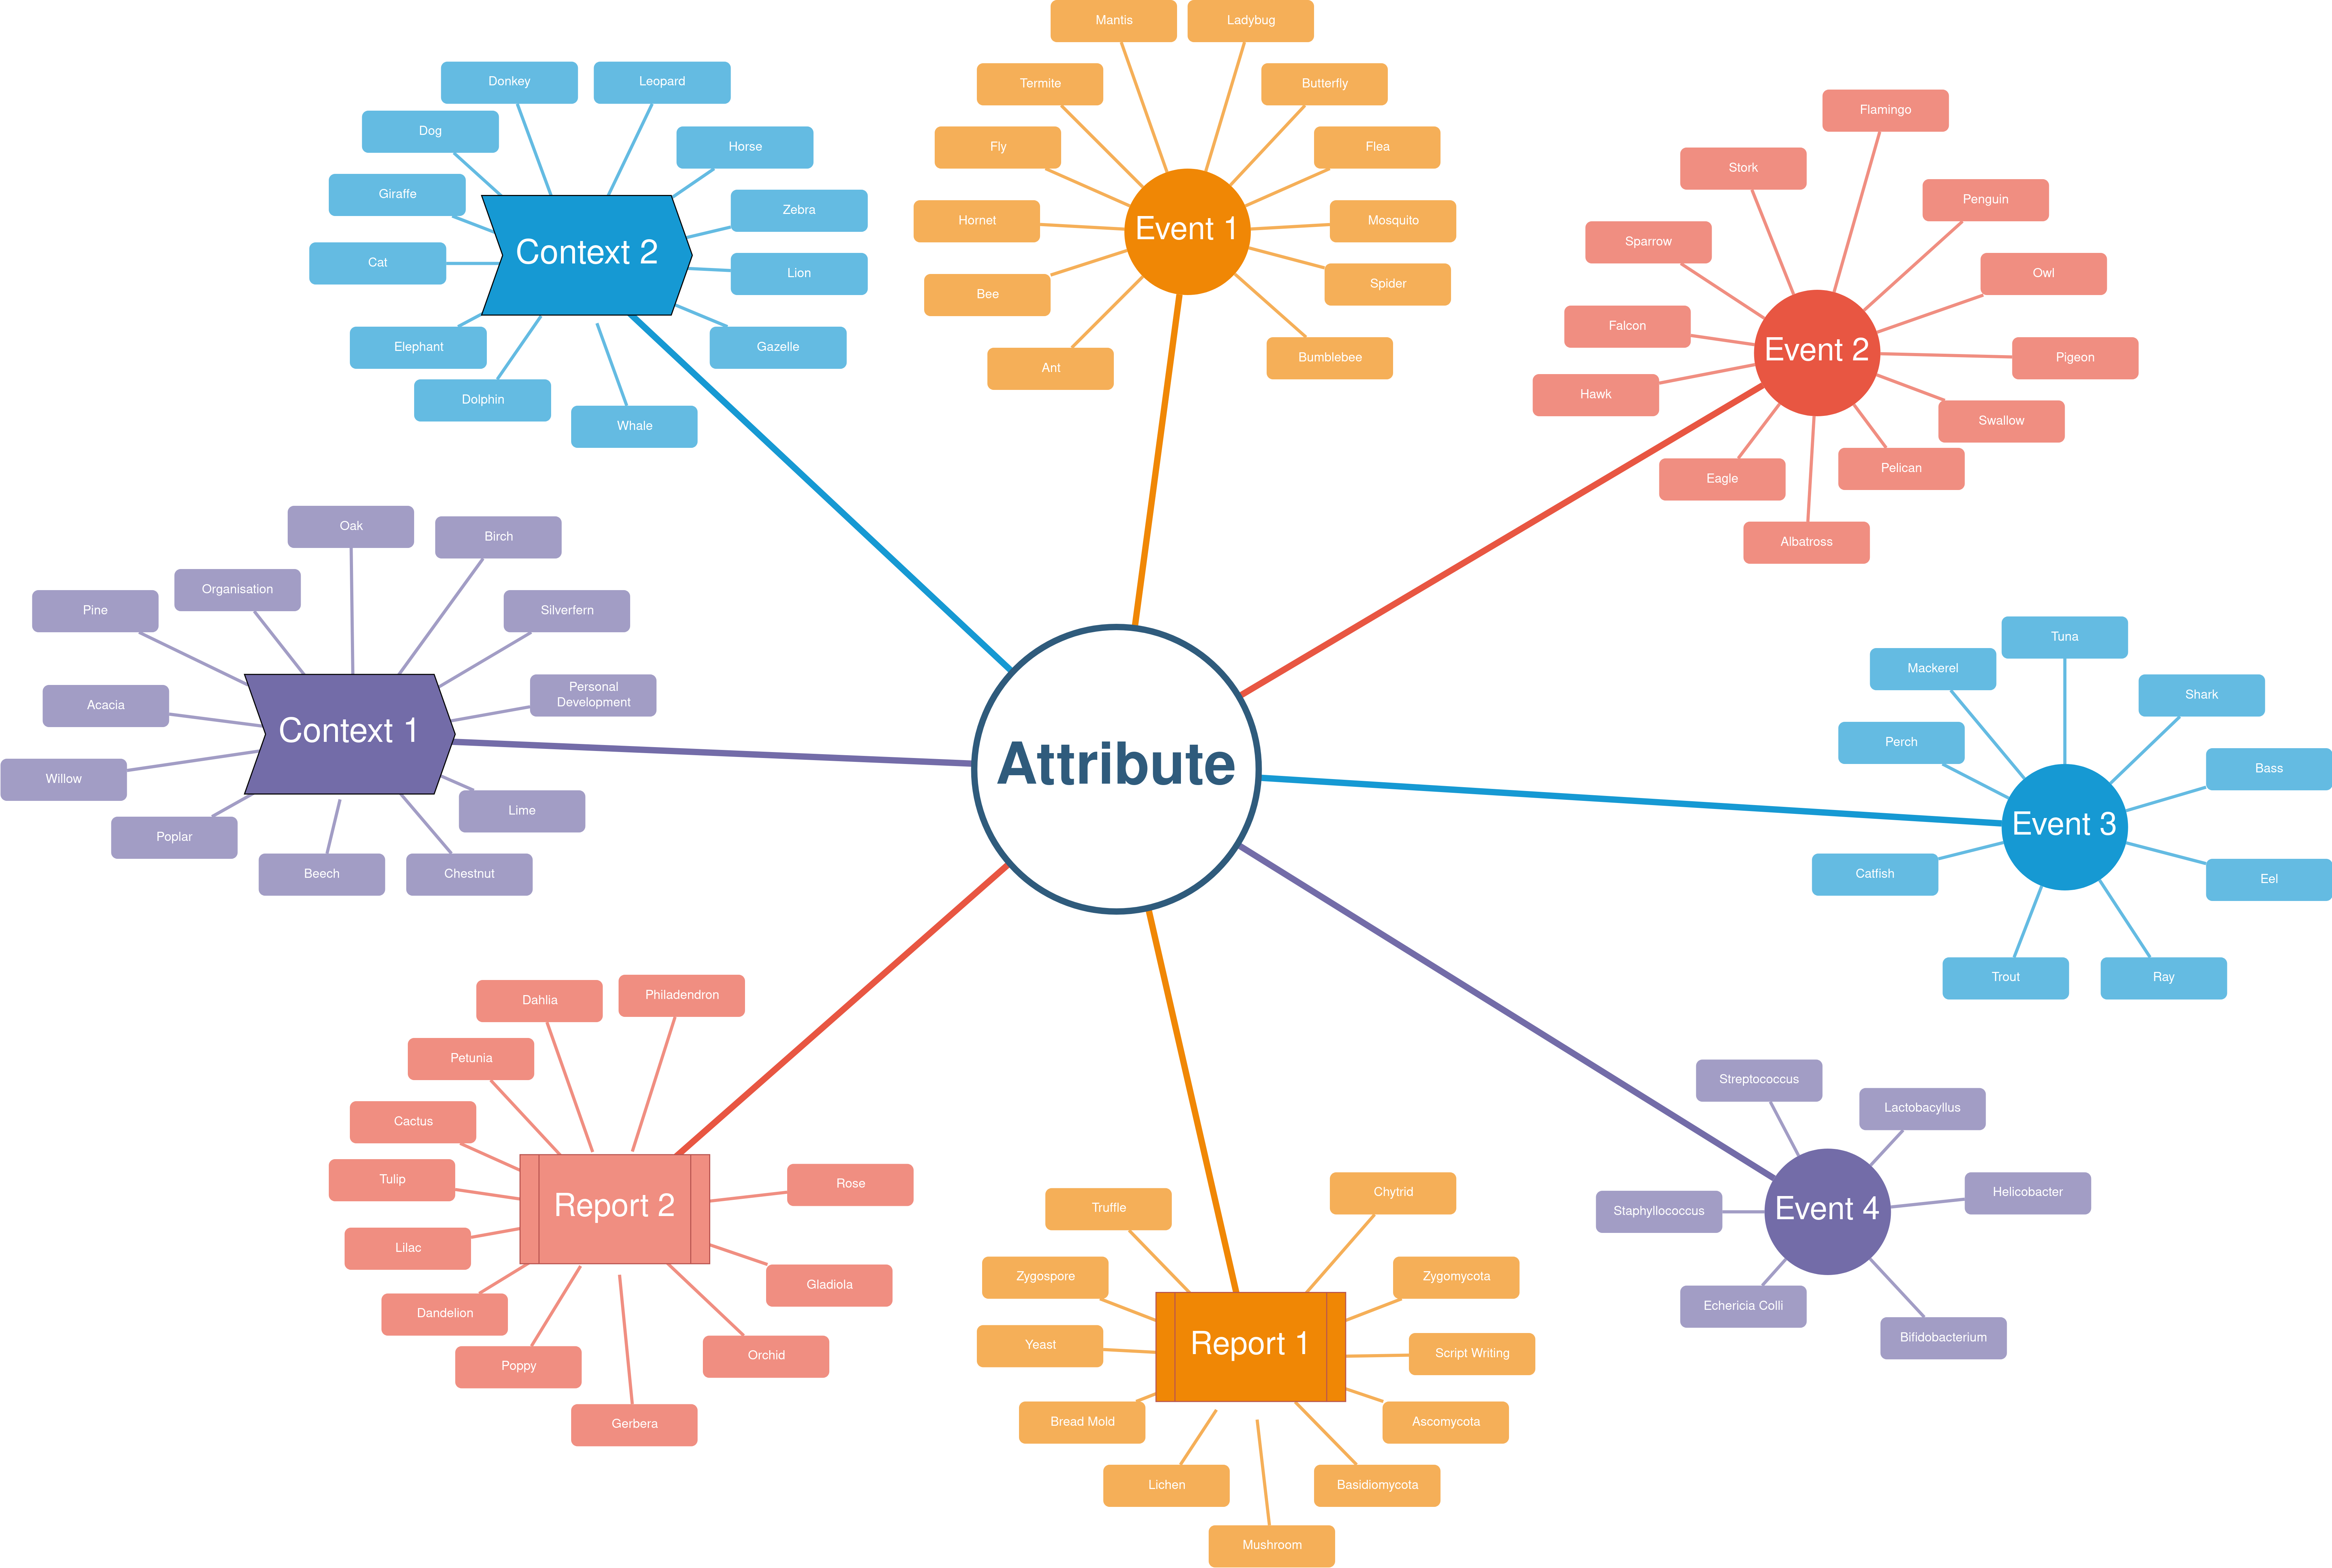
\includegraphics[width=0.7\linewidth]{pictures/attribute-centric.png}
    \end{center}
\end{frame}

\begin{frame}
    \frametitle{> Redefine how we interact with data II}
    \begin{itemize}
        \item Unified search mechanics
        \begin{itemize}
            \item Code deduplication
            \item Streamlined way to search for data
            \item Opening up the full power of the API searches to UI users
            \item Translation layer for the deprecated endpoints
        \end{itemize}
    \end{itemize}
    \begin{center}
        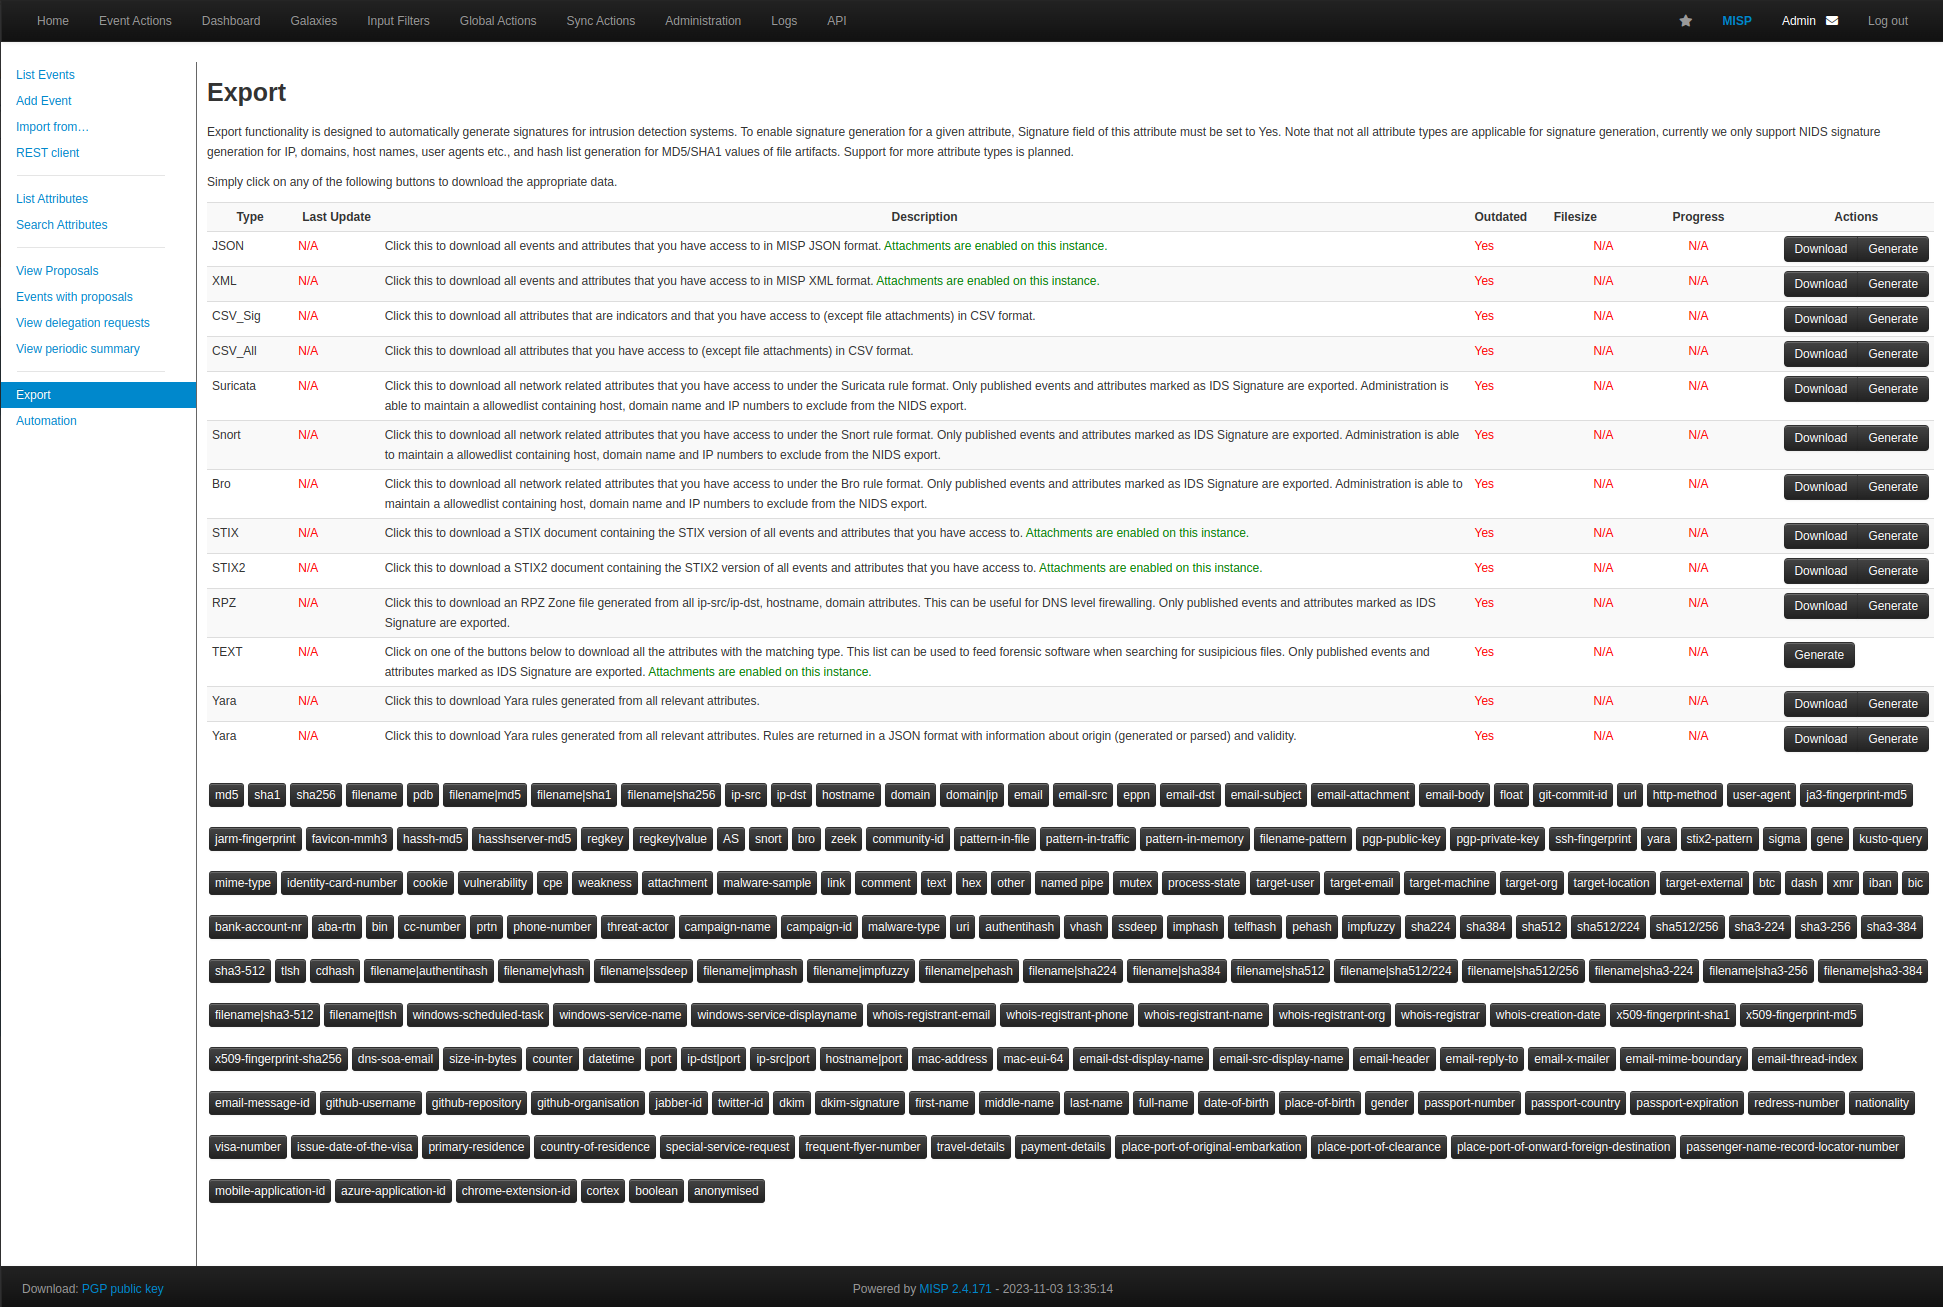
\includegraphics[width=0.7\linewidth]{pictures/misp-export.png}
    \end{center}
\end{frame}

\begin{frame}
    \frametitle{> Redefine how we interact with data III}
    \begin{itemize}
        \item Refactor the Event view
        \begin{itemize}
            \item Key Elements at first glance
            \item Emphasis on the context (Insights, Taxonomies, Galaxies, Correlation, $\cdot$)
            \item Massive performance gains by moving to the composition of separate atomic endpoints
            \item Sneak peak ? \faIcon{smile}
        \end{itemize}
    \end{itemize}
\end{frame}

\begin{frame}
    \frametitle{Sneak peak of the new Event view - WiP}
    \begin{center}
        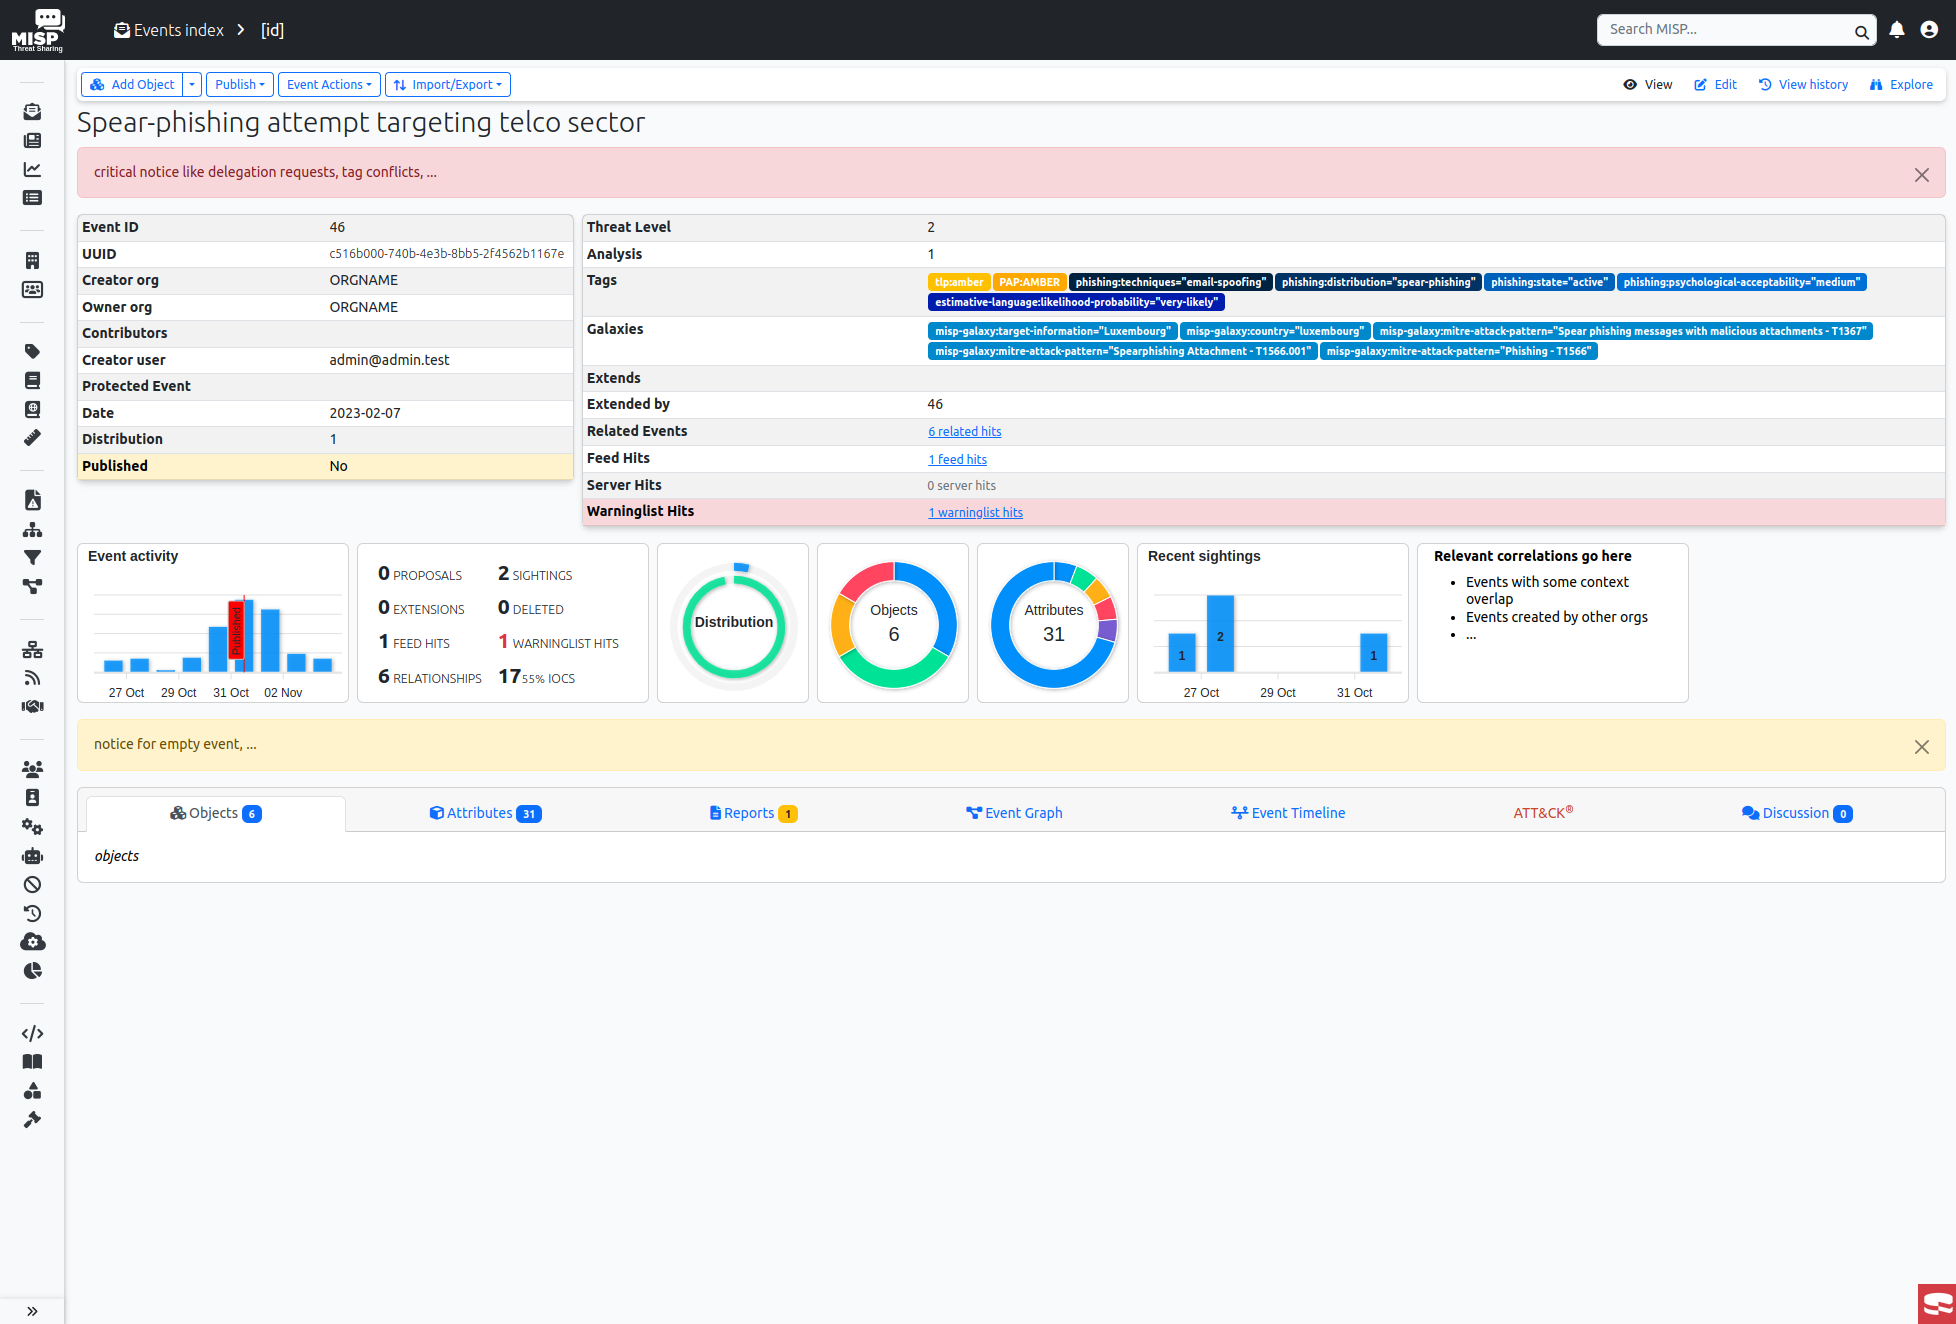
\includegraphics[width=1.0\linewidth]{pictures/event-view.png}
    \end{center}
\end{frame}


\section{Considerations}
\begin{frame}
    \frametitle{> MISP Core format}
    \vspace{-5em}
    \begin{center}
        
\includegraphics[width=0.35\linewidth]{pictures/misp-standard.png}
    \end{center}
    \vspace{1em}
    \begin{itemize}
        \item Created in \textbf{2012}, Officially became a standard in 2016
        \item \textbf{No breaking changes} since its birth, And we'll maintain this streak
        \item Format will keep evolving to support new functionalities
    \end{itemize}
\end{frame}

\begin{frame}
    \frametitle{> API Compatibility}
    \begin{itemize}
        \item The aim is to achieve a \textbf{near 100\% compatibility} with the old API
        \item "Near" only due to the functionalities removed as a result of deprecation.
        \item Strategy: Mapping with a translation layer
    \end{itemize}
    \begin{center}
        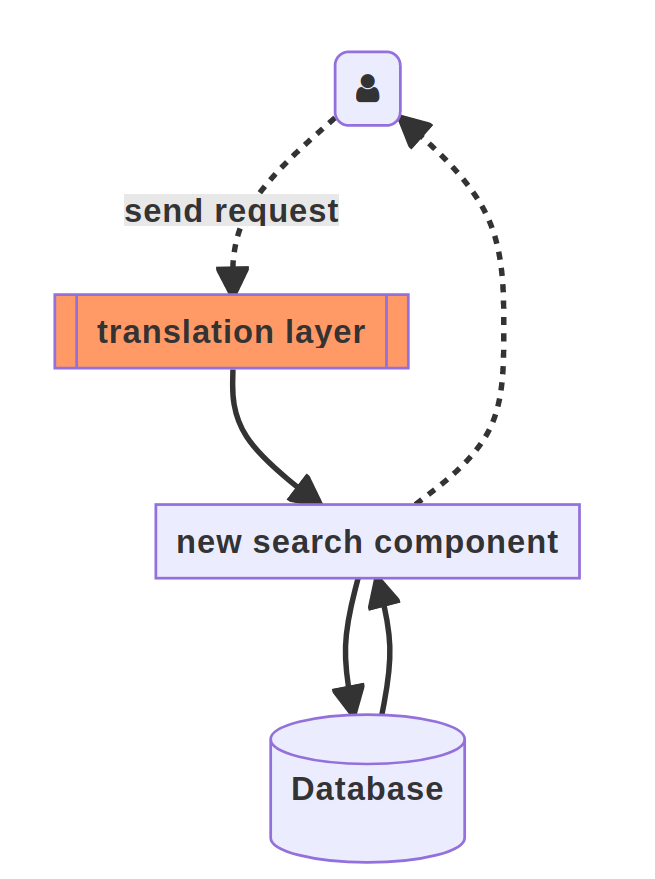
\includegraphics[width=0.35\linewidth]{pictures/api-translation.png}
    \end{center}
\end{frame}

\begin{frame}
    \frametitle{> Synchronisation compatibility}
    \begin{itemize}
        \item API Compatibility means Synchronisation compatibility
        \item MISP 3 servers will be able to sync with MISP 2.4 and vice versa
    \end{itemize}
    \begin{center}
        \textbf{\large BUT}
    \end{center}
    \begin{itemize}
        \item MISP \textbf{2.4} $\rightarrow$ \textbf{3}
        \begin{itemize}
            \item Full support
        \end{itemize}
        \item MISP \textbf{3} $\rightarrow$ \textbf{2.4}
        \begin{itemize}
            \item Lossy when sharing new types of datapoints
            \item E.g: Tags on Objects
        \end{itemize}
    \end{itemize}
\end{frame}

\begin{frame}
    \frametitle{> Support for MISP 2.4}
    \vspace{-1em}
    \begin{center}
        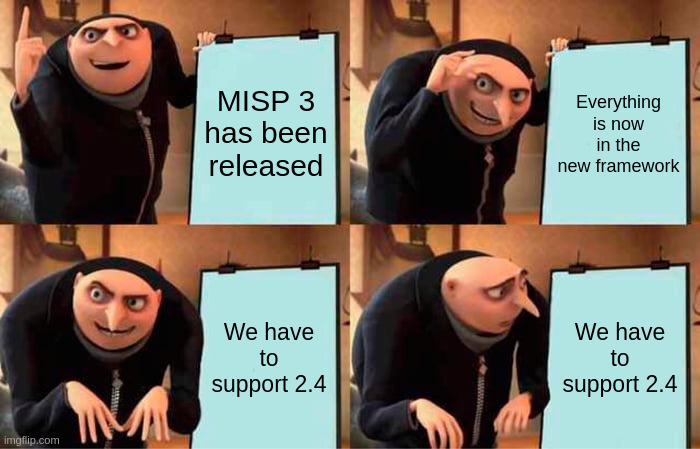
\includegraphics[width=0.7\linewidth]{pictures/support-for-2.jpeg}
    \end{center}
    \vspace{-1em}
    \begin{itemize}
        \item MISP 2.4 will be \textbf{supported for a limited time}
        \item \textbf{6 months} support post MISP 3 release
        \begin{itemize}
            \item Potential changes/improvements on 2.4 to better support MISP 3 interactions
        \end{itemize}
    \end{itemize}
\end{frame}

\begin{frame}
    \frametitle{> Migration support for 2.4 $\rightarrow$ 3}
    \begin{center}
        
\includegraphics[width=0.40\linewidth]{pictures/update}
    \end{center}
    \begin{itemize}
        \item No one-click update; manual script execution required
        \item Migration tools will be included in MISP 3 to help you
        \item This allows us to make underlaying changes such as
        \begin{itemize}
            \item Database changes
            \item Libraries changes (e.g supervisor in favour of cake-resque)
        \end{itemize}
    \end{itemize}
\end{frame}

\begin{frame}
    \frametitle{> Installation for new instances}
    \begin{minipage}{0.52\textwidth}
        \begin{itemize}
            \item \textbf{Simplified} installation based on package managers
            \item Upstream Docker installer
            \item OS targerts: \textbf{Ubuntu} and \textbf{RHEL}
        \end{itemize}
    \end{minipage}%
    \begin{minipage}{0.48\textwidth}
        \begin{center}
            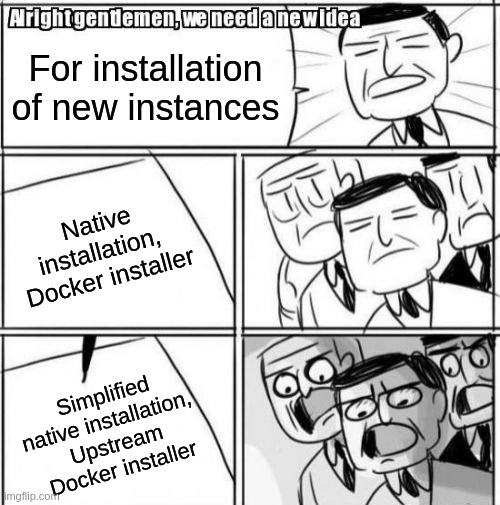
\includegraphics[width=0.99\linewidth]{pictures/new-installation.jpeg}
        \end{center}
    \end{minipage}
\end{frame}

\begin{frame}
    \begin{center}
        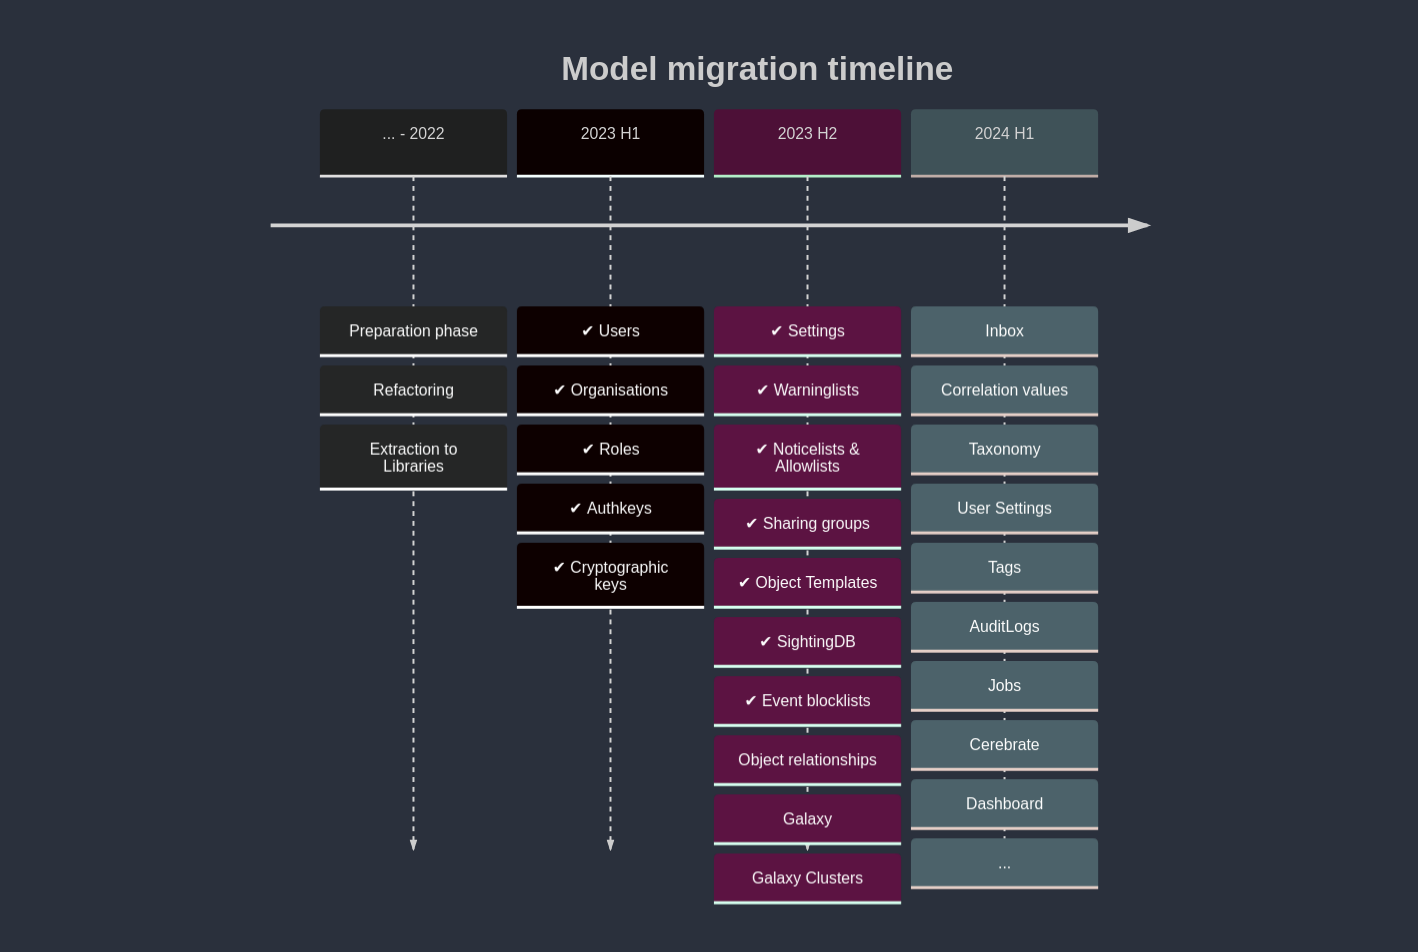
\includegraphics[width=0.99\linewidth]{pictures/timeline.png}
    \end{center}
\end{frame}

\begin{frame}
    \frametitle{> Our hopes and expectations for the FIRST community}
    \begin{center}
        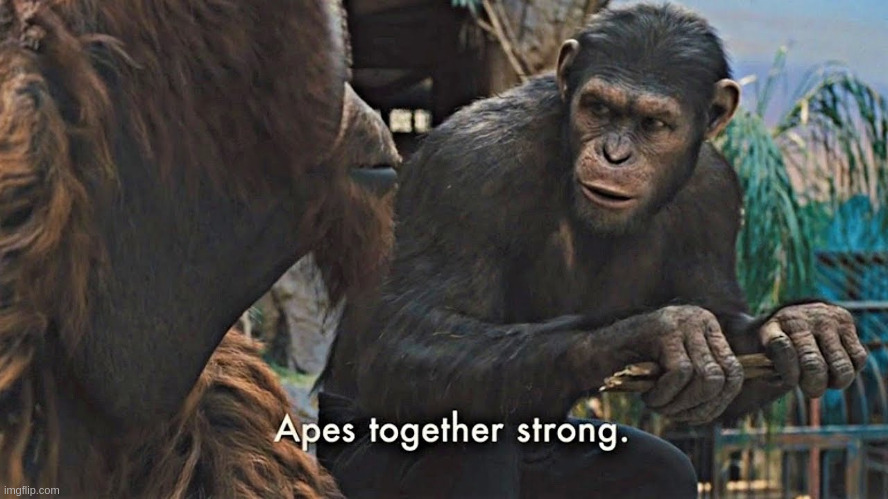
\includegraphics[width=0.50\linewidth]{pictures/apes-together-strong.jpeg}
    \end{center}
    \begin{itemize}
        \item We will list features marked for culling
        \begin{itemize}
            \item If you're using any of them, please let us know!
        \end{itemize}
        \item We will be lauching a beta phase in the future
        \begin{itemize}
            \item Feedback \& improvements are more than welcome!
        \end{itemize}
        \item Want to get involved?
        \begin{itemize}
            \item 
\includegraphics[width=4em]{pictures/3x-branch.png} 3-x branch - \texttt{\scriptsize MISP/MISP/tree/3.x}
            \item \faIcon{chalkboard-teacher} Project for migration - \texttt{\scriptsize github.com/orgs/MISP/projects/2}
        \end{itemize}
    \end{itemize}
\end{frame}
